\begin{figure}[H] \centering % Created by tikzDevice version 0.12.4 on 2023-08-13 18:11:37
% !TEX encoding = UTF-8 Unicode
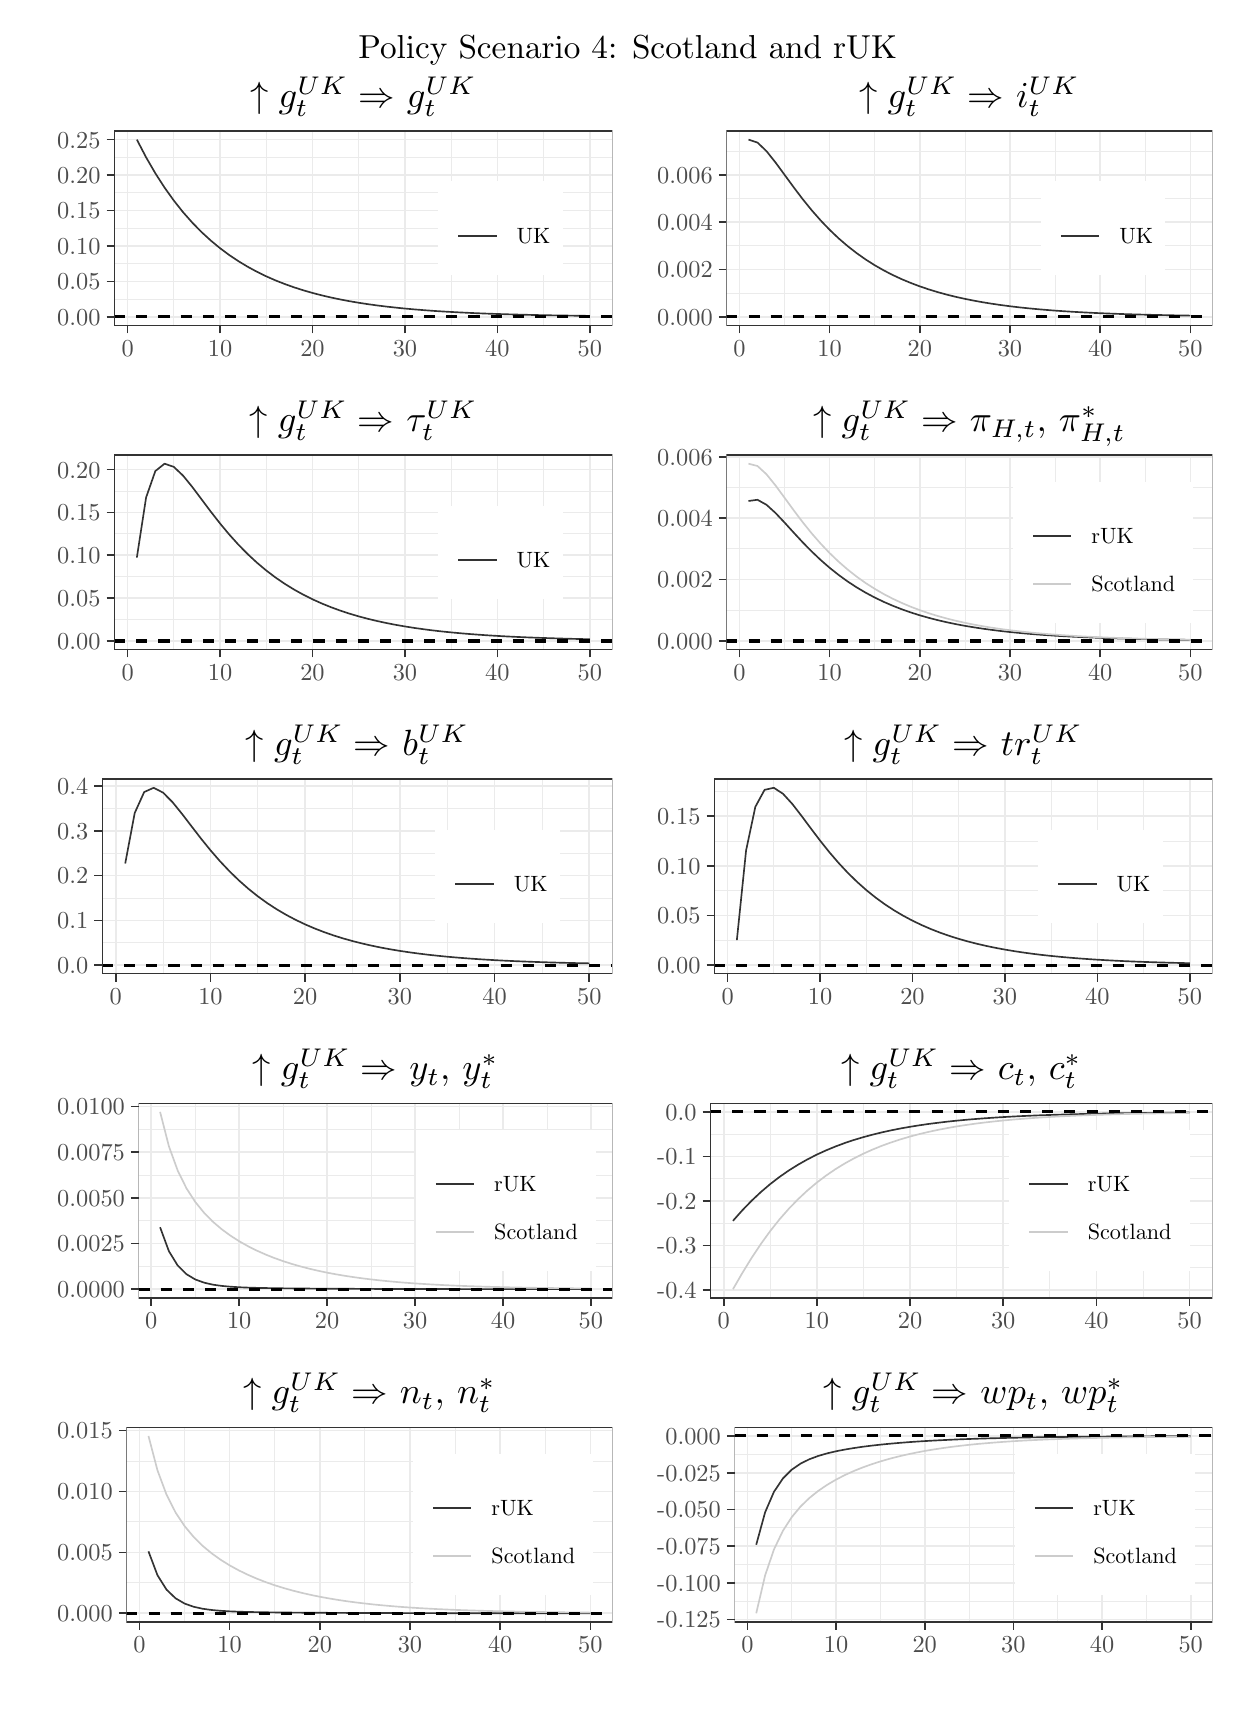
\begin{tikzpicture}[x=1pt,y=1pt]
\definecolor{fillColor}{RGB}{255,255,255}
\path[use as bounding box,fill=fillColor,fill opacity=0.00] (0,0) rectangle (433.62,599.84);
\begin{scope}
\path[clip] (  0.00,468.44) rectangle (216.81,585.55);
\definecolor{drawColor}{RGB}{255,255,255}
\definecolor{fillColor}{RGB}{255,255,255}

\path[draw=drawColor,line width= 0.6pt,line join=round,line cap=round,fill=fillColor] (  0.00,468.44) rectangle (216.81,585.55);
\end{scope}
\begin{scope}
\path[clip] ( 31.27,492.12) rectangle (211.31,562.59);
\definecolor{fillColor}{RGB}{255,255,255}

\path[fill=fillColor] ( 31.27,492.12) rectangle (211.31,562.59);
\definecolor{drawColor}{gray}{0.92}

\path[draw=drawColor,line width= 0.3pt,line join=round] ( 31.27,501.73) --
	(211.31,501.73);

\path[draw=drawColor,line width= 0.3pt,line join=round] ( 31.27,514.54) --
	(211.31,514.54);

\path[draw=drawColor,line width= 0.3pt,line join=round] ( 31.27,527.36) --
	(211.31,527.36);

\path[draw=drawColor,line width= 0.3pt,line join=round] ( 31.27,540.17) --
	(211.31,540.17);

\path[draw=drawColor,line width= 0.3pt,line join=round] ( 31.27,552.98) --
	(211.31,552.98);

\path[draw=drawColor,line width= 0.3pt,line join=round] ( 52.81,492.12) --
	( 52.81,562.59);

\path[draw=drawColor,line width= 0.3pt,line join=round] ( 86.22,492.12) --
	( 86.22,562.59);

\path[draw=drawColor,line width= 0.3pt,line join=round] (119.62,492.12) --
	(119.62,562.59);

\path[draw=drawColor,line width= 0.3pt,line join=round] (153.02,492.12) --
	(153.02,562.59);

\path[draw=drawColor,line width= 0.3pt,line join=round] (186.43,492.12) --
	(186.43,562.59);

\path[draw=drawColor,line width= 0.6pt,line join=round] ( 31.27,495.32) --
	(211.31,495.32);

\path[draw=drawColor,line width= 0.6pt,line join=round] ( 31.27,508.14) --
	(211.31,508.14);

\path[draw=drawColor,line width= 0.6pt,line join=round] ( 31.27,520.95) --
	(211.31,520.95);

\path[draw=drawColor,line width= 0.6pt,line join=round] ( 31.27,533.76) --
	(211.31,533.76);

\path[draw=drawColor,line width= 0.6pt,line join=round] ( 31.27,546.58) --
	(211.31,546.58);

\path[draw=drawColor,line width= 0.6pt,line join=round] ( 31.27,559.39) --
	(211.31,559.39);

\path[draw=drawColor,line width= 0.6pt,line join=round] ( 36.11,492.12) --
	( 36.11,562.59);

\path[draw=drawColor,line width= 0.6pt,line join=round] ( 69.52,492.12) --
	( 69.52,562.59);

\path[draw=drawColor,line width= 0.6pt,line join=round] (102.92,492.12) --
	(102.92,562.59);

\path[draw=drawColor,line width= 0.6pt,line join=round] (136.32,492.12) --
	(136.32,562.59);

\path[draw=drawColor,line width= 0.6pt,line join=round] (169.72,492.12) --
	(169.72,562.59);

\path[draw=drawColor,line width= 0.6pt,line join=round] (203.13,492.12) --
	(203.13,562.59);
\definecolor{drawColor}{gray}{0.20}

\path[draw=drawColor,line width= 0.6pt,line join=round] ( 39.45,559.39) --
	( 42.79,552.98) --
	( 46.13,547.22) --
	( 49.47,542.03) --
	( 52.81,537.36) --
	( 56.15,533.15) --
	( 59.50,529.37) --
	( 62.84,525.96) --
	( 66.18,522.90) --
	( 69.52,520.14) --
	( 72.86,517.66) --
	( 76.20,515.43) --
	( 79.54,513.42) --
	( 82.88,511.61) --
	( 86.22,509.98) --
	( 89.56,508.51) --
	( 92.90,507.20) --
	( 96.24,506.01) --
	( 99.58,504.94) --
	(102.92,503.98) --
	(106.26,503.11) --
	(109.60,502.33) --
	(112.94,501.63) --
	(116.28,501.00) --
	(119.62,500.43) --
	(122.96,499.92) --
	(126.30,499.46) --
	(129.64,499.05) --
	(132.98,498.68) --
	(136.32,498.34) --
	(139.66,498.04) --
	(143.00,497.77) --
	(146.34,497.52) --
	(149.68,497.30) --
	(153.02,497.11) --
	(156.36,496.93) --
	(159.70,496.77) --
	(163.04,496.62) --
	(166.38,496.49) --
	(169.72,496.38) --
	(173.06,496.27) --
	(176.40,496.18) --
	(179.74,496.09) --
	(183.08,496.01) --
	(186.43,495.94) --
	(189.77,495.88) --
	(193.11,495.83) --
	(196.45,495.78) --
	(199.79,495.73) --
	(203.13,495.69);
\definecolor{drawColor}{RGB}{0,0,0}

\path[draw=drawColor,line width= 1.1pt,dash pattern=on 4pt off 4pt ,line join=round] ( 31.27,495.32) -- (211.31,495.32);
\definecolor{drawColor}{gray}{0.20}

\path[draw=drawColor,line width= 0.6pt,line join=round,line cap=round] ( 31.27,492.12) rectangle (211.31,562.59);
\end{scope}
\begin{scope}
\path[clip] (  0.00,  0.00) rectangle (433.62,599.84);
\definecolor{drawColor}{gray}{0.30}

\node[text=drawColor,anchor=base east,inner sep=0pt, outer sep=0pt, scale=  0.88] at ( 26.32,492.29) {0.00};

\node[text=drawColor,anchor=base east,inner sep=0pt, outer sep=0pt, scale=  0.88] at ( 26.32,505.11) {0.05};

\node[text=drawColor,anchor=base east,inner sep=0pt, outer sep=0pt, scale=  0.88] at ( 26.32,517.92) {0.10};

\node[text=drawColor,anchor=base east,inner sep=0pt, outer sep=0pt, scale=  0.88] at ( 26.32,530.73) {0.15};

\node[text=drawColor,anchor=base east,inner sep=0pt, outer sep=0pt, scale=  0.88] at ( 26.32,543.55) {0.20};

\node[text=drawColor,anchor=base east,inner sep=0pt, outer sep=0pt, scale=  0.88] at ( 26.32,556.36) {0.25};
\end{scope}
\begin{scope}
\path[clip] (  0.00,  0.00) rectangle (433.62,599.84);
\definecolor{drawColor}{gray}{0.20}

\path[draw=drawColor,line width= 0.6pt,line join=round] ( 28.52,495.32) --
	( 31.27,495.32);

\path[draw=drawColor,line width= 0.6pt,line join=round] ( 28.52,508.14) --
	( 31.27,508.14);

\path[draw=drawColor,line width= 0.6pt,line join=round] ( 28.52,520.95) --
	( 31.27,520.95);

\path[draw=drawColor,line width= 0.6pt,line join=round] ( 28.52,533.76) --
	( 31.27,533.76);

\path[draw=drawColor,line width= 0.6pt,line join=round] ( 28.52,546.58) --
	( 31.27,546.58);

\path[draw=drawColor,line width= 0.6pt,line join=round] ( 28.52,559.39) --
	( 31.27,559.39);
\end{scope}
\begin{scope}
\path[clip] (  0.00,  0.00) rectangle (433.62,599.84);
\definecolor{drawColor}{gray}{0.20}

\path[draw=drawColor,line width= 0.6pt,line join=round] ( 36.11,489.37) --
	( 36.11,492.12);

\path[draw=drawColor,line width= 0.6pt,line join=round] ( 69.52,489.37) --
	( 69.52,492.12);

\path[draw=drawColor,line width= 0.6pt,line join=round] (102.92,489.37) --
	(102.92,492.12);

\path[draw=drawColor,line width= 0.6pt,line join=round] (136.32,489.37) --
	(136.32,492.12);

\path[draw=drawColor,line width= 0.6pt,line join=round] (169.72,489.37) --
	(169.72,492.12);

\path[draw=drawColor,line width= 0.6pt,line join=round] (203.13,489.37) --
	(203.13,492.12);
\end{scope}
\begin{scope}
\path[clip] (  0.00,  0.00) rectangle (433.62,599.84);
\definecolor{drawColor}{gray}{0.30}

\node[text=drawColor,anchor=base,inner sep=0pt, outer sep=0pt, scale=  0.88] at ( 36.11,481.11) {0};

\node[text=drawColor,anchor=base,inner sep=0pt, outer sep=0pt, scale=  0.88] at ( 69.52,481.11) {10};

\node[text=drawColor,anchor=base,inner sep=0pt, outer sep=0pt, scale=  0.88] at (102.92,481.11) {20};

\node[text=drawColor,anchor=base,inner sep=0pt, outer sep=0pt, scale=  0.88] at (136.32,481.11) {30};

\node[text=drawColor,anchor=base,inner sep=0pt, outer sep=0pt, scale=  0.88] at (169.72,481.11) {40};

\node[text=drawColor,anchor=base,inner sep=0pt, outer sep=0pt, scale=  0.88] at (203.13,481.11) {50};
\end{scope}
\begin{scope}
\path[clip] (  0.00,  0.00) rectangle (433.62,599.84);
\definecolor{fillColor}{RGB}{255,255,255}

\path[fill=fillColor] (148.30,510.43) rectangle (193.30,544.28);
\end{scope}
\begin{scope}
\path[clip] (  0.00,  0.00) rectangle (433.62,599.84);
\definecolor{fillColor}{RGB}{255,255,255}

\path[fill=fillColor] (153.80,515.93) rectangle (171.15,533.28);
\end{scope}
\begin{scope}
\path[clip] (  0.00,  0.00) rectangle (433.62,599.84);
\definecolor{drawColor}{gray}{0.20}

\path[draw=drawColor,line width= 0.6pt,line join=round] (155.54,524.61) -- (169.41,524.61);
\end{scope}
\begin{scope}
\path[clip] (  0.00,  0.00) rectangle (433.62,599.84);
\definecolor{drawColor}{RGB}{0,0,0}

\node[text=drawColor,anchor=base west,inner sep=0pt, outer sep=0pt, scale=  0.80] at (176.65,521.85) {UK};
\end{scope}
\begin{scope}
\path[clip] (  0.00,  0.00) rectangle (433.62,599.84);
\definecolor{drawColor}{RGB}{0,0,0}

\node[text=drawColor,anchor=base,inner sep=0pt, outer sep=0pt, scale=  1.32] at (121.29,570.96) {$\uparrow  g^{UK}_t \Rightarrow $ ${g^{UK}_t}$};
\end{scope}
\begin{scope}
\path[clip] (216.81,468.44) rectangle (433.62,585.55);
\definecolor{drawColor}{RGB}{255,255,255}
\definecolor{fillColor}{RGB}{255,255,255}

\path[draw=drawColor,line width= 0.6pt,line join=round,line cap=round,fill=fillColor] (216.81,468.44) rectangle (433.62,585.55);
\end{scope}
\begin{scope}
\path[clip] (252.48,492.12) rectangle (428.12,562.59);
\definecolor{fillColor}{RGB}{255,255,255}

\path[fill=fillColor] (252.48,492.12) rectangle (428.12,562.59);
\definecolor{drawColor}{gray}{0.92}

\path[draw=drawColor,line width= 0.3pt,line join=round] (252.48,503.88) --
	(428.12,503.88);

\path[draw=drawColor,line width= 0.3pt,line join=round] (252.48,521.00) --
	(428.12,521.00);

\path[draw=drawColor,line width= 0.3pt,line join=round] (252.48,538.12) --
	(428.12,538.12);

\path[draw=drawColor,line width= 0.3pt,line join=round] (252.48,555.24) --
	(428.12,555.24);

\path[draw=drawColor,line width= 0.3pt,line join=round] (273.50,492.12) --
	(273.50,562.59);

\path[draw=drawColor,line width= 0.3pt,line join=round] (306.08,492.12) --
	(306.08,562.59);

\path[draw=drawColor,line width= 0.3pt,line join=round] (338.67,492.12) --
	(338.67,562.59);

\path[draw=drawColor,line width= 0.3pt,line join=round] (371.26,492.12) --
	(371.26,562.59);

\path[draw=drawColor,line width= 0.3pt,line join=round] (403.84,492.12) --
	(403.84,562.59);

\path[draw=drawColor,line width= 0.6pt,line join=round] (252.48,495.32) --
	(428.12,495.32);

\path[draw=drawColor,line width= 0.6pt,line join=round] (252.48,512.44) --
	(428.12,512.44);

\path[draw=drawColor,line width= 0.6pt,line join=round] (252.48,529.56) --
	(428.12,529.56);

\path[draw=drawColor,line width= 0.6pt,line join=round] (252.48,546.68) --
	(428.12,546.68);

\path[draw=drawColor,line width= 0.6pt,line join=round] (257.20,492.12) --
	(257.20,562.59);

\path[draw=drawColor,line width= 0.6pt,line join=round] (289.79,492.12) --
	(289.79,562.59);

\path[draw=drawColor,line width= 0.6pt,line join=round] (322.38,492.12) --
	(322.38,562.59);

\path[draw=drawColor,line width= 0.6pt,line join=round] (354.96,492.12) --
	(354.96,562.59);

\path[draw=drawColor,line width= 0.6pt,line join=round] (387.55,492.12) --
	(387.55,562.59);

\path[draw=drawColor,line width= 0.6pt,line join=round] (420.14,492.12) --
	(420.14,562.59);
\definecolor{drawColor}{gray}{0.20}

\path[draw=drawColor,line width= 0.6pt,line join=round] (260.46,559.39) --
	(263.72,558.32) --
	(266.98,555.20) --
	(270.24,551.11) --
	(273.50,546.67) --
	(276.76,542.21) --
	(280.01,537.92) --
	(283.27,533.90) --
	(286.53,530.19) --
	(289.79,526.79) --
	(293.05,523.69) --
	(296.31,520.89) --
	(299.57,518.35) --
	(302.82,516.06) --
	(306.08,513.99) --
	(309.34,512.13) --
	(312.60,510.45) --
	(315.86,508.94) --
	(319.12,507.58) --
	(322.38,506.35) --
	(325.64,505.25) --
	(328.89,504.26) --
	(332.15,503.36) --
	(335.41,502.56) --
	(338.67,501.84) --
	(341.93,501.19) --
	(345.19,500.60) --
	(348.45,500.07) --
	(351.70,499.60) --
	(354.96,499.17) --
	(358.22,498.78) --
	(361.48,498.44) --
	(364.74,498.13) --
	(368.00,497.85) --
	(371.26,497.59) --
	(374.52,497.37) --
	(377.77,497.16) --
	(381.03,496.98) --
	(384.29,496.81) --
	(387.55,496.66) --
	(390.81,496.53) --
	(394.07,496.41) --
	(397.33,496.30) --
	(400.58,496.20) --
	(403.84,496.12) --
	(407.10,496.04) --
	(410.36,495.97) --
	(413.62,495.90) --
	(416.88,495.84) --
	(420.14,495.79);
\definecolor{drawColor}{RGB}{0,0,0}

\path[draw=drawColor,line width= 1.1pt,dash pattern=on 4pt off 4pt ,line join=round] (252.48,495.32) -- (428.12,495.32);
\definecolor{drawColor}{gray}{0.20}

\path[draw=drawColor,line width= 0.6pt,line join=round,line cap=round] (252.48,492.12) rectangle (428.12,562.59);
\end{scope}
\begin{scope}
\path[clip] (  0.00,  0.00) rectangle (433.62,599.84);
\definecolor{drawColor}{gray}{0.30}

\node[text=drawColor,anchor=base east,inner sep=0pt, outer sep=0pt, scale=  0.88] at (247.53,492.29) {0.000};

\node[text=drawColor,anchor=base east,inner sep=0pt, outer sep=0pt, scale=  0.88] at (247.53,509.41) {0.002};

\node[text=drawColor,anchor=base east,inner sep=0pt, outer sep=0pt, scale=  0.88] at (247.53,526.53) {0.004};

\node[text=drawColor,anchor=base east,inner sep=0pt, outer sep=0pt, scale=  0.88] at (247.53,543.65) {0.006};
\end{scope}
\begin{scope}
\path[clip] (  0.00,  0.00) rectangle (433.62,599.84);
\definecolor{drawColor}{gray}{0.20}

\path[draw=drawColor,line width= 0.6pt,line join=round] (249.73,495.32) --
	(252.48,495.32);

\path[draw=drawColor,line width= 0.6pt,line join=round] (249.73,512.44) --
	(252.48,512.44);

\path[draw=drawColor,line width= 0.6pt,line join=round] (249.73,529.56) --
	(252.48,529.56);

\path[draw=drawColor,line width= 0.6pt,line join=round] (249.73,546.68) --
	(252.48,546.68);
\end{scope}
\begin{scope}
\path[clip] (  0.00,  0.00) rectangle (433.62,599.84);
\definecolor{drawColor}{gray}{0.20}

\path[draw=drawColor,line width= 0.6pt,line join=round] (257.20,489.37) --
	(257.20,492.12);

\path[draw=drawColor,line width= 0.6pt,line join=round] (289.79,489.37) --
	(289.79,492.12);

\path[draw=drawColor,line width= 0.6pt,line join=round] (322.38,489.37) --
	(322.38,492.12);

\path[draw=drawColor,line width= 0.6pt,line join=round] (354.96,489.37) --
	(354.96,492.12);

\path[draw=drawColor,line width= 0.6pt,line join=round] (387.55,489.37) --
	(387.55,492.12);

\path[draw=drawColor,line width= 0.6pt,line join=round] (420.14,489.37) --
	(420.14,492.12);
\end{scope}
\begin{scope}
\path[clip] (  0.00,  0.00) rectangle (433.62,599.84);
\definecolor{drawColor}{gray}{0.30}

\node[text=drawColor,anchor=base,inner sep=0pt, outer sep=0pt, scale=  0.88] at (257.20,481.11) {0};

\node[text=drawColor,anchor=base,inner sep=0pt, outer sep=0pt, scale=  0.88] at (289.79,481.11) {10};

\node[text=drawColor,anchor=base,inner sep=0pt, outer sep=0pt, scale=  0.88] at (322.38,481.11) {20};

\node[text=drawColor,anchor=base,inner sep=0pt, outer sep=0pt, scale=  0.88] at (354.96,481.11) {30};

\node[text=drawColor,anchor=base,inner sep=0pt, outer sep=0pt, scale=  0.88] at (387.55,481.11) {40};

\node[text=drawColor,anchor=base,inner sep=0pt, outer sep=0pt, scale=  0.88] at (420.14,481.11) {50};
\end{scope}
\begin{scope}
\path[clip] (  0.00,  0.00) rectangle (433.62,599.84);
\definecolor{fillColor}{RGB}{255,255,255}

\path[fill=fillColor] (366.10,510.43) rectangle (411.10,544.28);
\end{scope}
\begin{scope}
\path[clip] (  0.00,  0.00) rectangle (433.62,599.84);
\definecolor{fillColor}{RGB}{255,255,255}

\path[fill=fillColor] (371.60,515.93) rectangle (388.95,533.28);
\end{scope}
\begin{scope}
\path[clip] (  0.00,  0.00) rectangle (433.62,599.84);
\definecolor{drawColor}{gray}{0.20}

\path[draw=drawColor,line width= 0.6pt,line join=round] (373.34,524.61) -- (387.21,524.61);
\end{scope}
\begin{scope}
\path[clip] (  0.00,  0.00) rectangle (433.62,599.84);
\definecolor{drawColor}{RGB}{0,0,0}

\node[text=drawColor,anchor=base west,inner sep=0pt, outer sep=0pt, scale=  0.80] at (394.45,521.85) {UK};
\end{scope}
\begin{scope}
\path[clip] (  0.00,  0.00) rectangle (433.62,599.84);
\definecolor{drawColor}{RGB}{0,0,0}

\node[text=drawColor,anchor=base,inner sep=0pt, outer sep=0pt, scale=  1.32] at (340.30,570.96) {$\uparrow  g^{UK}_t \Rightarrow $ ${i^{UK}_t}$};
\end{scope}
\begin{scope}
\path[clip] (  0.00,351.33) rectangle (216.81,468.44);
\definecolor{drawColor}{RGB}{255,255,255}
\definecolor{fillColor}{RGB}{255,255,255}

\path[draw=drawColor,line width= 0.6pt,line join=round,line cap=round,fill=fillColor] (  0.00,351.33) rectangle (216.81,468.44);
\end{scope}
\begin{scope}
\path[clip] ( 31.27,375.01) rectangle (211.31,445.48);
\definecolor{fillColor}{RGB}{255,255,255}

\path[fill=fillColor] ( 31.27,375.01) rectangle (211.31,445.48);
\definecolor{drawColor}{gray}{0.92}

\path[draw=drawColor,line width= 0.3pt,line join=round] ( 31.27,385.95) --
	(211.31,385.95);

\path[draw=drawColor,line width= 0.3pt,line join=round] ( 31.27,401.43) --
	(211.31,401.43);

\path[draw=drawColor,line width= 0.3pt,line join=round] ( 31.27,416.92) --
	(211.31,416.92);

\path[draw=drawColor,line width= 0.3pt,line join=round] ( 31.27,432.40) --
	(211.31,432.40);

\path[draw=drawColor,line width= 0.3pt,line join=round] ( 52.81,375.01) --
	( 52.81,445.48);

\path[draw=drawColor,line width= 0.3pt,line join=round] ( 86.22,375.01) --
	( 86.22,445.48);

\path[draw=drawColor,line width= 0.3pt,line join=round] (119.62,375.01) --
	(119.62,445.48);

\path[draw=drawColor,line width= 0.3pt,line join=round] (153.02,375.01) --
	(153.02,445.48);

\path[draw=drawColor,line width= 0.3pt,line join=round] (186.43,375.01) --
	(186.43,445.48);

\path[draw=drawColor,line width= 0.6pt,line join=round] ( 31.27,378.21) --
	(211.31,378.21);

\path[draw=drawColor,line width= 0.6pt,line join=round] ( 31.27,393.69) --
	(211.31,393.69);

\path[draw=drawColor,line width= 0.6pt,line join=round] ( 31.27,409.18) --
	(211.31,409.18);

\path[draw=drawColor,line width= 0.6pt,line join=round] ( 31.27,424.66) --
	(211.31,424.66);

\path[draw=drawColor,line width= 0.6pt,line join=round] ( 31.27,440.14) --
	(211.31,440.14);

\path[draw=drawColor,line width= 0.6pt,line join=round] ( 36.11,375.01) --
	( 36.11,445.48);

\path[draw=drawColor,line width= 0.6pt,line join=round] ( 69.52,375.01) --
	( 69.52,445.48);

\path[draw=drawColor,line width= 0.6pt,line join=round] (102.92,375.01) --
	(102.92,445.48);

\path[draw=drawColor,line width= 0.6pt,line join=round] (136.32,375.01) --
	(136.32,445.48);

\path[draw=drawColor,line width= 0.6pt,line join=round] (169.72,375.01) --
	(169.72,445.48);

\path[draw=drawColor,line width= 0.6pt,line join=round] (203.13,375.01) --
	(203.13,445.48);
\definecolor{drawColor}{gray}{0.20}

\path[draw=drawColor,line width= 0.6pt,line join=round] ( 39.45,408.34) --
	( 42.79,430.06) --
	( 46.13,439.62) --
	( 49.47,442.28) --
	( 52.81,441.12) --
	( 56.15,437.96) --
	( 59.50,433.85) --
	( 62.84,429.40) --
	( 66.18,424.94) --
	( 69.52,420.67) --
	( 72.86,416.66) --
	( 76.20,412.96) --
	( 79.54,409.57) --
	( 82.88,406.48) --
	( 86.22,403.68) --
	( 89.56,401.15) --
	( 92.90,398.87) --
	( 96.24,396.81) --
	( 99.58,394.96) --
	(102.92,393.28) --
	(106.26,391.78) --
	(109.60,390.42) --
	(112.94,389.20) --
	(116.28,388.10) --
	(119.62,387.11) --
	(122.96,386.22) --
	(126.30,385.42) --
	(129.64,384.70) --
	(132.98,384.05) --
	(136.32,383.47) --
	(139.66,382.94) --
	(143.00,382.47) --
	(146.34,382.04) --
	(149.68,381.66) --
	(153.02,381.32) --
	(156.36,381.01) --
	(159.70,380.73) --
	(163.04,380.48) --
	(166.38,380.25) --
	(169.72,380.05) --
	(173.06,379.86) --
	(176.40,379.70) --
	(179.74,379.55) --
	(183.08,379.42) --
	(186.43,379.30) --
	(189.77,379.19) --
	(193.11,379.09) --
	(196.45,379.00) --
	(199.79,378.92) --
	(203.13,378.85);
\definecolor{drawColor}{RGB}{0,0,0}

\path[draw=drawColor,line width= 1.1pt,dash pattern=on 4pt off 4pt ,line join=round] ( 31.27,378.21) -- (211.31,378.21);
\definecolor{drawColor}{gray}{0.20}

\path[draw=drawColor,line width= 0.6pt,line join=round,line cap=round] ( 31.27,375.01) rectangle (211.31,445.48);
\end{scope}
\begin{scope}
\path[clip] (  0.00,  0.00) rectangle (433.62,599.84);
\definecolor{drawColor}{gray}{0.30}

\node[text=drawColor,anchor=base east,inner sep=0pt, outer sep=0pt, scale=  0.88] at ( 26.32,375.18) {0.00};

\node[text=drawColor,anchor=base east,inner sep=0pt, outer sep=0pt, scale=  0.88] at ( 26.32,390.66) {0.05};

\node[text=drawColor,anchor=base east,inner sep=0pt, outer sep=0pt, scale=  0.88] at ( 26.32,406.15) {0.10};

\node[text=drawColor,anchor=base east,inner sep=0pt, outer sep=0pt, scale=  0.88] at ( 26.32,421.63) {0.15};

\node[text=drawColor,anchor=base east,inner sep=0pt, outer sep=0pt, scale=  0.88] at ( 26.32,437.11) {0.20};
\end{scope}
\begin{scope}
\path[clip] (  0.00,  0.00) rectangle (433.62,599.84);
\definecolor{drawColor}{gray}{0.20}

\path[draw=drawColor,line width= 0.6pt,line join=round] ( 28.52,378.21) --
	( 31.27,378.21);

\path[draw=drawColor,line width= 0.6pt,line join=round] ( 28.52,393.69) --
	( 31.27,393.69);

\path[draw=drawColor,line width= 0.6pt,line join=round] ( 28.52,409.18) --
	( 31.27,409.18);

\path[draw=drawColor,line width= 0.6pt,line join=round] ( 28.52,424.66) --
	( 31.27,424.66);

\path[draw=drawColor,line width= 0.6pt,line join=round] ( 28.52,440.14) --
	( 31.27,440.14);
\end{scope}
\begin{scope}
\path[clip] (  0.00,  0.00) rectangle (433.62,599.84);
\definecolor{drawColor}{gray}{0.20}

\path[draw=drawColor,line width= 0.6pt,line join=round] ( 36.11,372.26) --
	( 36.11,375.01);

\path[draw=drawColor,line width= 0.6pt,line join=round] ( 69.52,372.26) --
	( 69.52,375.01);

\path[draw=drawColor,line width= 0.6pt,line join=round] (102.92,372.26) --
	(102.92,375.01);

\path[draw=drawColor,line width= 0.6pt,line join=round] (136.32,372.26) --
	(136.32,375.01);

\path[draw=drawColor,line width= 0.6pt,line join=round] (169.72,372.26) --
	(169.72,375.01);

\path[draw=drawColor,line width= 0.6pt,line join=round] (203.13,372.26) --
	(203.13,375.01);
\end{scope}
\begin{scope}
\path[clip] (  0.00,  0.00) rectangle (433.62,599.84);
\definecolor{drawColor}{gray}{0.30}

\node[text=drawColor,anchor=base,inner sep=0pt, outer sep=0pt, scale=  0.88] at ( 36.11,364.00) {0};

\node[text=drawColor,anchor=base,inner sep=0pt, outer sep=0pt, scale=  0.88] at ( 69.52,364.00) {10};

\node[text=drawColor,anchor=base,inner sep=0pt, outer sep=0pt, scale=  0.88] at (102.92,364.00) {20};

\node[text=drawColor,anchor=base,inner sep=0pt, outer sep=0pt, scale=  0.88] at (136.32,364.00) {30};

\node[text=drawColor,anchor=base,inner sep=0pt, outer sep=0pt, scale=  0.88] at (169.72,364.00) {40};

\node[text=drawColor,anchor=base,inner sep=0pt, outer sep=0pt, scale=  0.88] at (203.13,364.00) {50};
\end{scope}
\begin{scope}
\path[clip] (  0.00,  0.00) rectangle (433.62,599.84);
\definecolor{fillColor}{RGB}{255,255,255}

\path[fill=fillColor] (148.30,393.32) rectangle (193.30,427.17);
\end{scope}
\begin{scope}
\path[clip] (  0.00,  0.00) rectangle (433.62,599.84);
\definecolor{fillColor}{RGB}{255,255,255}

\path[fill=fillColor] (153.80,398.82) rectangle (171.15,416.17);
\end{scope}
\begin{scope}
\path[clip] (  0.00,  0.00) rectangle (433.62,599.84);
\definecolor{drawColor}{gray}{0.20}

\path[draw=drawColor,line width= 0.6pt,line join=round] (155.54,407.50) -- (169.41,407.50);
\end{scope}
\begin{scope}
\path[clip] (  0.00,  0.00) rectangle (433.62,599.84);
\definecolor{drawColor}{RGB}{0,0,0}

\node[text=drawColor,anchor=base west,inner sep=0pt, outer sep=0pt, scale=  0.80] at (176.65,404.74) {UK};
\end{scope}
\begin{scope}
\path[clip] (  0.00,  0.00) rectangle (433.62,599.84);
\definecolor{drawColor}{RGB}{0,0,0}

\node[text=drawColor,anchor=base,inner sep=0pt, outer sep=0pt, scale=  1.32] at (121.29,453.85) {$\uparrow  g^{UK}_t \Rightarrow $ ${\tau^{UK}_t}$};
\end{scope}
\begin{scope}
\path[clip] (216.81,351.33) rectangle (433.62,468.44);
\definecolor{drawColor}{RGB}{255,255,255}
\definecolor{fillColor}{RGB}{255,255,255}

\path[draw=drawColor,line width= 0.6pt,line join=round,line cap=round,fill=fillColor] (216.81,351.33) rectangle (433.62,468.44);
\end{scope}
\begin{scope}
\path[clip] (252.48,375.01) rectangle (428.12,445.48);
\definecolor{fillColor}{RGB}{255,255,255}

\path[fill=fillColor] (252.48,375.01) rectangle (428.12,445.48);
\definecolor{drawColor}{gray}{0.92}

\path[draw=drawColor,line width= 0.3pt,line join=round] (252.48,389.31) --
	(428.12,389.31);

\path[draw=drawColor,line width= 0.3pt,line join=round] (252.48,411.51) --
	(428.12,411.51);

\path[draw=drawColor,line width= 0.3pt,line join=round] (252.48,433.71) --
	(428.12,433.71);

\path[draw=drawColor,line width= 0.3pt,line join=round] (273.50,375.01) --
	(273.50,445.48);

\path[draw=drawColor,line width= 0.3pt,line join=round] (306.08,375.01) --
	(306.08,445.48);

\path[draw=drawColor,line width= 0.3pt,line join=round] (338.67,375.01) --
	(338.67,445.48);

\path[draw=drawColor,line width= 0.3pt,line join=round] (371.26,375.01) --
	(371.26,445.48);

\path[draw=drawColor,line width= 0.3pt,line join=round] (403.84,375.01) --
	(403.84,445.48);

\path[draw=drawColor,line width= 0.6pt,line join=round] (252.48,378.21) --
	(428.12,378.21);

\path[draw=drawColor,line width= 0.6pt,line join=round] (252.48,400.41) --
	(428.12,400.41);

\path[draw=drawColor,line width= 0.6pt,line join=round] (252.48,422.61) --
	(428.12,422.61);

\path[draw=drawColor,line width= 0.6pt,line join=round] (252.48,444.81) --
	(428.12,444.81);

\path[draw=drawColor,line width= 0.6pt,line join=round] (257.20,375.01) --
	(257.20,445.48);

\path[draw=drawColor,line width= 0.6pt,line join=round] (289.79,375.01) --
	(289.79,445.48);

\path[draw=drawColor,line width= 0.6pt,line join=round] (322.38,375.01) --
	(322.38,445.48);

\path[draw=drawColor,line width= 0.6pt,line join=round] (354.96,375.01) --
	(354.96,445.48);

\path[draw=drawColor,line width= 0.6pt,line join=round] (387.55,375.01) --
	(387.55,445.48);

\path[draw=drawColor,line width= 0.6pt,line join=round] (420.14,375.01) --
	(420.14,445.48);
\definecolor{drawColor}{gray}{0.20}

\path[draw=drawColor,line width= 0.6pt,line join=round] (260.46,428.80) --
	(263.72,429.24) --
	(266.98,427.42) --
	(270.24,424.46) --
	(273.50,421.00) --
	(276.76,417.42) --
	(280.01,413.91) --
	(283.27,410.59) --
	(286.53,407.50) --
	(289.79,404.66) --
	(293.05,402.07) --
	(296.31,399.71) --
	(299.57,397.58) --
	(302.82,395.66) --
	(306.08,393.92) --
	(309.34,392.35) --
	(312.60,390.94) --
	(315.86,389.67) --
	(319.12,388.52) --
	(322.38,387.49) --
	(325.64,386.57) --
	(328.89,385.73) --
	(332.15,384.98) --
	(335.41,384.30) --
	(338.67,383.69) --
	(341.93,383.15) --
	(345.19,382.65) --
	(348.45,382.21) --
	(351.70,381.81) --
	(354.96,381.45) --
	(358.22,381.13) --
	(361.48,380.83) --
	(364.74,380.57) --
	(368.00,380.34) --
	(371.26,380.12) --
	(374.52,379.93) --
	(377.77,379.76) --
	(381.03,379.61) --
	(384.29,379.47) --
	(387.55,379.34) --
	(390.81,379.23) --
	(394.07,379.13) --
	(397.33,379.04) --
	(400.58,378.95) --
	(403.84,378.88) --
	(407.10,378.81) --
	(410.36,378.75) --
	(413.62,378.70) --
	(416.88,378.65) --
	(420.14,378.61);
\definecolor{drawColor}{gray}{0.80}

\path[draw=drawColor,line width= 0.6pt,line join=round] (260.46,442.28) --
	(263.72,441.44) --
	(266.98,438.44) --
	(270.24,434.40) --
	(273.50,429.97) --
	(276.76,425.50) --
	(280.01,421.19) --
	(283.27,417.14) --
	(286.53,413.40) --
	(289.79,409.97) --
	(293.05,406.85) --
	(296.31,404.02) --
	(299.57,401.45) --
	(302.82,399.14) --
	(306.08,397.06) --
	(309.34,395.17) --
	(312.60,393.48) --
	(315.86,391.96) --
	(319.12,390.58) --
	(322.38,389.35) --
	(325.64,388.23) --
	(328.89,387.23) --
	(332.15,386.33) --
	(335.41,385.52) --
	(338.67,384.79) --
	(341.93,384.13) --
	(345.19,383.54) --
	(348.45,383.01) --
	(351.70,382.53) --
	(354.96,382.10) --
	(358.22,381.71) --
	(361.48,381.36) --
	(364.74,381.04) --
	(368.00,380.76) --
	(371.26,380.51) --
	(374.52,380.28) --
	(377.77,380.07) --
	(381.03,379.88) --
	(384.29,379.72) --
	(387.55,379.57) --
	(390.81,379.43) --
	(394.07,379.31) --
	(397.33,379.20) --
	(400.58,379.10) --
	(403.84,379.01) --
	(407.10,378.93) --
	(410.36,378.86) --
	(413.62,378.80) --
	(416.88,378.74) --
	(420.14,378.68);
\definecolor{drawColor}{RGB}{0,0,0}

\path[draw=drawColor,line width= 1.1pt,dash pattern=on 4pt off 4pt ,line join=round] (252.48,378.21) -- (428.12,378.21);
\definecolor{drawColor}{gray}{0.20}

\path[draw=drawColor,line width= 0.6pt,line join=round,line cap=round] (252.48,375.01) rectangle (428.12,445.48);
\end{scope}
\begin{scope}
\path[clip] (  0.00,  0.00) rectangle (433.62,599.84);
\definecolor{drawColor}{gray}{0.30}

\node[text=drawColor,anchor=base east,inner sep=0pt, outer sep=0pt, scale=  0.88] at (247.53,375.18) {0.000};

\node[text=drawColor,anchor=base east,inner sep=0pt, outer sep=0pt, scale=  0.88] at (247.53,397.38) {0.002};

\node[text=drawColor,anchor=base east,inner sep=0pt, outer sep=0pt, scale=  0.88] at (247.53,419.58) {0.004};

\node[text=drawColor,anchor=base east,inner sep=0pt, outer sep=0pt, scale=  0.88] at (247.53,441.78) {0.006};
\end{scope}
\begin{scope}
\path[clip] (  0.00,  0.00) rectangle (433.62,599.84);
\definecolor{drawColor}{gray}{0.20}

\path[draw=drawColor,line width= 0.6pt,line join=round] (249.73,378.21) --
	(252.48,378.21);

\path[draw=drawColor,line width= 0.6pt,line join=round] (249.73,400.41) --
	(252.48,400.41);

\path[draw=drawColor,line width= 0.6pt,line join=round] (249.73,422.61) --
	(252.48,422.61);

\path[draw=drawColor,line width= 0.6pt,line join=round] (249.73,444.81) --
	(252.48,444.81);
\end{scope}
\begin{scope}
\path[clip] (  0.00,  0.00) rectangle (433.62,599.84);
\definecolor{drawColor}{gray}{0.20}

\path[draw=drawColor,line width= 0.6pt,line join=round] (257.20,372.26) --
	(257.20,375.01);

\path[draw=drawColor,line width= 0.6pt,line join=round] (289.79,372.26) --
	(289.79,375.01);

\path[draw=drawColor,line width= 0.6pt,line join=round] (322.38,372.26) --
	(322.38,375.01);

\path[draw=drawColor,line width= 0.6pt,line join=round] (354.96,372.26) --
	(354.96,375.01);

\path[draw=drawColor,line width= 0.6pt,line join=round] (387.55,372.26) --
	(387.55,375.01);

\path[draw=drawColor,line width= 0.6pt,line join=round] (420.14,372.26) --
	(420.14,375.01);
\end{scope}
\begin{scope}
\path[clip] (  0.00,  0.00) rectangle (433.62,599.84);
\definecolor{drawColor}{gray}{0.30}

\node[text=drawColor,anchor=base,inner sep=0pt, outer sep=0pt, scale=  0.88] at (257.20,364.00) {0};

\node[text=drawColor,anchor=base,inner sep=0pt, outer sep=0pt, scale=  0.88] at (289.79,364.00) {10};

\node[text=drawColor,anchor=base,inner sep=0pt, outer sep=0pt, scale=  0.88] at (322.38,364.00) {20};

\node[text=drawColor,anchor=base,inner sep=0pt, outer sep=0pt, scale=  0.88] at (354.96,364.00) {30};

\node[text=drawColor,anchor=base,inner sep=0pt, outer sep=0pt, scale=  0.88] at (387.55,364.00) {40};

\node[text=drawColor,anchor=base,inner sep=0pt, outer sep=0pt, scale=  0.88] at (420.14,364.00) {50};
\end{scope}
\begin{scope}
\path[clip] (  0.00,  0.00) rectangle (433.62,599.84);
\definecolor{fillColor}{RGB}{255,255,255}

\path[fill=fillColor] (356.06,384.65) rectangle (421.15,435.84);
\end{scope}
\begin{scope}
\path[clip] (  0.00,  0.00) rectangle (433.62,599.84);
\definecolor{fillColor}{RGB}{255,255,255}

\path[fill=fillColor] (361.56,407.50) rectangle (378.90,424.84);
\end{scope}
\begin{scope}
\path[clip] (  0.00,  0.00) rectangle (433.62,599.84);
\definecolor{drawColor}{gray}{0.20}

\path[draw=drawColor,line width= 0.6pt,line join=round] (363.29,416.17) -- (377.17,416.17);
\end{scope}
\begin{scope}
\path[clip] (  0.00,  0.00) rectangle (433.62,599.84);
\definecolor{fillColor}{RGB}{255,255,255}

\path[fill=fillColor] (361.56,390.15) rectangle (378.90,407.50);
\end{scope}
\begin{scope}
\path[clip] (  0.00,  0.00) rectangle (433.62,599.84);
\definecolor{drawColor}{gray}{0.80}

\path[draw=drawColor,line width= 0.6pt,line join=round] (363.29,398.82) -- (377.17,398.82);
\end{scope}
\begin{scope}
\path[clip] (  0.00,  0.00) rectangle (433.62,599.84);
\definecolor{drawColor}{RGB}{0,0,0}

\node[text=drawColor,anchor=base west,inner sep=0pt, outer sep=0pt, scale=  0.80] at (384.40,413.41) {rUK};
\end{scope}
\begin{scope}
\path[clip] (  0.00,  0.00) rectangle (433.62,599.84);
\definecolor{drawColor}{RGB}{0,0,0}

\node[text=drawColor,anchor=base west,inner sep=0pt, outer sep=0pt, scale=  0.80] at (384.40,396.07) {Scotland};
\end{scope}
\begin{scope}
\path[clip] (  0.00,  0.00) rectangle (433.62,599.84);
\definecolor{drawColor}{RGB}{0,0,0}

\node[text=drawColor,anchor=base,inner sep=0pt, outer sep=0pt, scale=  1.32] at (340.30,453.85) {$\uparrow  g^{UK}_t \Rightarrow $ ${\pi_{H,t}}$, ${\pi^*_{H,t}}$};
\end{scope}
\begin{scope}
\path[clip] (  0.00,234.22) rectangle (216.81,351.33);
\definecolor{drawColor}{RGB}{255,255,255}
\definecolor{fillColor}{RGB}{255,255,255}

\path[draw=drawColor,line width= 0.6pt,line join=round,line cap=round,fill=fillColor] (  0.00,234.22) rectangle (216.81,351.33);
\end{scope}
\begin{scope}
\path[clip] ( 26.87,257.90) rectangle (211.31,328.37);
\definecolor{fillColor}{RGB}{255,255,255}

\path[fill=fillColor] ( 26.87,257.90) rectangle (211.31,328.37);
\definecolor{drawColor}{gray}{0.92}

\path[draw=drawColor,line width= 0.3pt,line join=round] ( 26.87,269.19) --
	(211.31,269.19);

\path[draw=drawColor,line width= 0.3pt,line join=round] ( 26.87,285.35) --
	(211.31,285.35);

\path[draw=drawColor,line width= 0.3pt,line join=round] ( 26.87,301.52) --
	(211.31,301.52);

\path[draw=drawColor,line width= 0.3pt,line join=round] ( 26.87,317.69) --
	(211.31,317.69);

\path[draw=drawColor,line width= 0.3pt,line join=round] ( 48.94,257.90) --
	( 48.94,328.37);

\path[draw=drawColor,line width= 0.3pt,line join=round] ( 83.16,257.90) --
	( 83.16,328.37);

\path[draw=drawColor,line width= 0.3pt,line join=round] (117.38,257.90) --
	(117.38,328.37);

\path[draw=drawColor,line width= 0.3pt,line join=round] (151.60,257.90) --
	(151.60,328.37);

\path[draw=drawColor,line width= 0.3pt,line join=round] (185.82,257.90) --
	(185.82,328.37);

\path[draw=drawColor,line width= 0.6pt,line join=round] ( 26.87,261.10) --
	(211.31,261.10);

\path[draw=drawColor,line width= 0.6pt,line join=round] ( 26.87,277.27) --
	(211.31,277.27);

\path[draw=drawColor,line width= 0.6pt,line join=round] ( 26.87,293.44) --
	(211.31,293.44);

\path[draw=drawColor,line width= 0.6pt,line join=round] ( 26.87,309.60) --
	(211.31,309.60);

\path[draw=drawColor,line width= 0.6pt,line join=round] ( 26.87,325.77) --
	(211.31,325.77);

\path[draw=drawColor,line width= 0.6pt,line join=round] ( 31.83,257.90) --
	( 31.83,328.37);

\path[draw=drawColor,line width= 0.6pt,line join=round] ( 66.05,257.90) --
	( 66.05,328.37);

\path[draw=drawColor,line width= 0.6pt,line join=round] (100.27,257.90) --
	(100.27,328.37);

\path[draw=drawColor,line width= 0.6pt,line join=round] (134.49,257.90) --
	(134.49,328.37);

\path[draw=drawColor,line width= 0.6pt,line join=round] (168.71,257.90) --
	(168.71,328.37);

\path[draw=drawColor,line width= 0.6pt,line join=round] (202.93,257.90) --
	(202.93,328.37);
\definecolor{drawColor}{gray}{0.20}

\path[draw=drawColor,line width= 0.6pt,line join=round] ( 35.25,297.82) --
	( 38.68,316.06) --
	( 42.10,323.63) --
	( 45.52,325.17) --
	( 48.94,323.41) --
	( 52.36,319.95) --
	( 55.79,315.72) --
	( 59.21,311.25) --
	( 62.63,306.82) --
	( 66.05,302.60) --
	( 69.47,298.66) --
	( 72.90,295.03) --
	( 76.32,291.71) --
	( 79.74,288.69) --
	( 83.16,285.96) --
	( 86.58,283.49) --
	( 90.00,281.26) --
	( 93.43,279.25) --
	( 96.85,277.44) --
	(100.27,275.81) --
	(103.69,274.34) --
	(107.11,273.02) --
	(110.54,271.82) --
	(113.96,270.75) --
	(117.38,269.79) --
	(120.80,268.92) --
	(124.22,268.14) --
	(127.65,267.43) --
	(131.07,266.80) --
	(134.49,266.23) --
	(137.91,265.72) --
	(141.33,265.26) --
	(144.75,264.84) --
	(148.18,264.47) --
	(151.60,264.13) --
	(155.02,263.83) --
	(158.44,263.56) --
	(161.86,263.31) --
	(165.29,263.09) --
	(168.71,262.89) --
	(172.13,262.71) --
	(175.55,262.55) --
	(178.97,262.41) --
	(182.40,262.28) --
	(185.82,262.16) --
	(189.24,262.05) --
	(192.66,261.96) --
	(196.08,261.87) --
	(199.50,261.79) --
	(202.93,261.73);
\definecolor{drawColor}{RGB}{0,0,0}

\path[draw=drawColor,line width= 1.1pt,dash pattern=on 4pt off 4pt ,line join=round] ( 26.87,261.10) -- (211.31,261.10);
\definecolor{drawColor}{gray}{0.20}

\path[draw=drawColor,line width= 0.6pt,line join=round,line cap=round] ( 26.87,257.90) rectangle (211.31,328.37);
\end{scope}
\begin{scope}
\path[clip] (  0.00,  0.00) rectangle (433.62,599.84);
\definecolor{drawColor}{gray}{0.30}

\node[text=drawColor,anchor=base east,inner sep=0pt, outer sep=0pt, scale=  0.88] at ( 21.92,258.07) {0.0};

\node[text=drawColor,anchor=base east,inner sep=0pt, outer sep=0pt, scale=  0.88] at ( 21.92,274.24) {0.1};

\node[text=drawColor,anchor=base east,inner sep=0pt, outer sep=0pt, scale=  0.88] at ( 21.92,290.41) {0.2};

\node[text=drawColor,anchor=base east,inner sep=0pt, outer sep=0pt, scale=  0.88] at ( 21.92,306.57) {0.3};

\node[text=drawColor,anchor=base east,inner sep=0pt, outer sep=0pt, scale=  0.88] at ( 21.92,322.74) {0.4};
\end{scope}
\begin{scope}
\path[clip] (  0.00,  0.00) rectangle (433.62,599.84);
\definecolor{drawColor}{gray}{0.20}

\path[draw=drawColor,line width= 0.6pt,line join=round] ( 24.12,261.10) --
	( 26.87,261.10);

\path[draw=drawColor,line width= 0.6pt,line join=round] ( 24.12,277.27) --
	( 26.87,277.27);

\path[draw=drawColor,line width= 0.6pt,line join=round] ( 24.12,293.44) --
	( 26.87,293.44);

\path[draw=drawColor,line width= 0.6pt,line join=round] ( 24.12,309.60) --
	( 26.87,309.60);

\path[draw=drawColor,line width= 0.6pt,line join=round] ( 24.12,325.77) --
	( 26.87,325.77);
\end{scope}
\begin{scope}
\path[clip] (  0.00,  0.00) rectangle (433.62,599.84);
\definecolor{drawColor}{gray}{0.20}

\path[draw=drawColor,line width= 0.6pt,line join=round] ( 31.83,255.15) --
	( 31.83,257.90);

\path[draw=drawColor,line width= 0.6pt,line join=round] ( 66.05,255.15) --
	( 66.05,257.90);

\path[draw=drawColor,line width= 0.6pt,line join=round] (100.27,255.15) --
	(100.27,257.90);

\path[draw=drawColor,line width= 0.6pt,line join=round] (134.49,255.15) --
	(134.49,257.90);

\path[draw=drawColor,line width= 0.6pt,line join=round] (168.71,255.15) --
	(168.71,257.90);

\path[draw=drawColor,line width= 0.6pt,line join=round] (202.93,255.15) --
	(202.93,257.90);
\end{scope}
\begin{scope}
\path[clip] (  0.00,  0.00) rectangle (433.62,599.84);
\definecolor{drawColor}{gray}{0.30}

\node[text=drawColor,anchor=base,inner sep=0pt, outer sep=0pt, scale=  0.88] at ( 31.83,246.89) {0};

\node[text=drawColor,anchor=base,inner sep=0pt, outer sep=0pt, scale=  0.88] at ( 66.05,246.89) {10};

\node[text=drawColor,anchor=base,inner sep=0pt, outer sep=0pt, scale=  0.88] at (100.27,246.89) {20};

\node[text=drawColor,anchor=base,inner sep=0pt, outer sep=0pt, scale=  0.88] at (134.49,246.89) {30};

\node[text=drawColor,anchor=base,inner sep=0pt, outer sep=0pt, scale=  0.88] at (168.71,246.89) {40};

\node[text=drawColor,anchor=base,inner sep=0pt, outer sep=0pt, scale=  0.88] at (202.93,246.89) {50};
\end{scope}
\begin{scope}
\path[clip] (  0.00,  0.00) rectangle (433.62,599.84);
\definecolor{fillColor}{RGB}{255,255,255}

\path[fill=fillColor] (147.31,276.21) rectangle (192.31,310.06);
\end{scope}
\begin{scope}
\path[clip] (  0.00,  0.00) rectangle (433.62,599.84);
\definecolor{fillColor}{RGB}{255,255,255}

\path[fill=fillColor] (152.81,281.71) rectangle (170.16,299.06);
\end{scope}
\begin{scope}
\path[clip] (  0.00,  0.00) rectangle (433.62,599.84);
\definecolor{drawColor}{gray}{0.20}

\path[draw=drawColor,line width= 0.6pt,line join=round] (154.55,290.38) -- (168.42,290.38);
\end{scope}
\begin{scope}
\path[clip] (  0.00,  0.00) rectangle (433.62,599.84);
\definecolor{drawColor}{RGB}{0,0,0}

\node[text=drawColor,anchor=base west,inner sep=0pt, outer sep=0pt, scale=  0.80] at (175.66,287.63) {UK};
\end{scope}
\begin{scope}
\path[clip] (  0.00,  0.00) rectangle (433.62,599.84);
\definecolor{drawColor}{RGB}{0,0,0}

\node[text=drawColor,anchor=base,inner sep=0pt, outer sep=0pt, scale=  1.32] at (119.09,336.74) {$\uparrow  g^{UK}_t \Rightarrow $ ${b^{UK}_t}$};
\end{scope}
\begin{scope}
\path[clip] (216.81,234.22) rectangle (433.62,351.33);
\definecolor{drawColor}{RGB}{255,255,255}
\definecolor{fillColor}{RGB}{255,255,255}

\path[draw=drawColor,line width= 0.6pt,line join=round,line cap=round,fill=fillColor] (216.81,234.22) rectangle (433.62,351.33);
\end{scope}
\begin{scope}
\path[clip] (248.08,257.90) rectangle (428.12,328.37);
\definecolor{fillColor}{RGB}{255,255,255}

\path[fill=fillColor] (248.08,257.90) rectangle (428.12,328.37);
\definecolor{drawColor}{gray}{0.92}

\path[draw=drawColor,line width= 0.3pt,line join=round] (248.08,270.06) --
	(428.12,270.06);

\path[draw=drawColor,line width= 0.3pt,line join=round] (248.08,287.98) --
	(428.12,287.98);

\path[draw=drawColor,line width= 0.3pt,line join=round] (248.08,305.90) --
	(428.12,305.90);

\path[draw=drawColor,line width= 0.3pt,line join=round] (248.08,323.82) --
	(428.12,323.82);

\path[draw=drawColor,line width= 0.3pt,line join=round] (269.62,257.90) --
	(269.62,328.37);

\path[draw=drawColor,line width= 0.3pt,line join=round] (303.03,257.90) --
	(303.03,328.37);

\path[draw=drawColor,line width= 0.3pt,line join=round] (336.43,257.90) --
	(336.43,328.37);

\path[draw=drawColor,line width= 0.3pt,line join=round] (369.83,257.90) --
	(369.83,328.37);

\path[draw=drawColor,line width= 0.3pt,line join=round] (403.24,257.90) --
	(403.24,328.37);

\path[draw=drawColor,line width= 0.6pt,line join=round] (248.08,261.10) --
	(428.12,261.10);

\path[draw=drawColor,line width= 0.6pt,line join=round] (248.08,279.02) --
	(428.12,279.02);

\path[draw=drawColor,line width= 0.6pt,line join=round] (248.08,296.94) --
	(428.12,296.94);

\path[draw=drawColor,line width= 0.6pt,line join=round] (248.08,314.86) --
	(428.12,314.86);

\path[draw=drawColor,line width= 0.6pt,line join=round] (252.92,257.90) --
	(252.92,328.37);

\path[draw=drawColor,line width= 0.6pt,line join=round] (286.33,257.90) --
	(286.33,328.37);

\path[draw=drawColor,line width= 0.6pt,line join=round] (319.73,257.90) --
	(319.73,328.37);

\path[draw=drawColor,line width= 0.6pt,line join=round] (353.13,257.90) --
	(353.13,328.37);

\path[draw=drawColor,line width= 0.6pt,line join=round] (386.53,257.90) --
	(386.53,328.37);

\path[draw=drawColor,line width= 0.6pt,line join=round] (419.94,257.90) --
	(419.94,328.37);
\definecolor{drawColor}{gray}{0.20}

\path[draw=drawColor,line width= 0.6pt,line join=round] (256.26,270.11) --
	(259.60,302.54) --
	(262.94,318.29) --
	(266.28,324.43) --
	(269.62,325.17) --
	(272.96,322.98) --
	(276.31,319.31) --
	(279.65,314.99) --
	(282.99,310.50) --
	(286.33,306.09) --
	(289.67,301.91) --
	(293.01,298.02) --
	(296.35,294.44) --
	(299.69,291.18) --
	(303.03,288.21) --
	(306.37,285.52) --
	(309.71,283.09) --
	(313.05,280.90) --
	(316.39,278.93) --
	(319.73,277.15) --
	(323.07,275.55) --
	(326.41,274.10) --
	(329.75,272.80) --
	(333.09,271.63) --
	(336.43,270.58) --
	(339.77,269.63) --
	(343.11,268.78) --
	(346.45,268.01) --
	(349.79,267.32) --
	(353.13,266.70) --
	(356.47,266.14) --
	(359.81,265.64) --
	(363.15,265.18) --
	(366.49,264.77) --
	(369.83,264.41) --
	(373.17,264.08) --
	(376.51,263.78) --
	(379.85,263.51) --
	(383.19,263.27) --
	(386.53,263.05) --
	(389.87,262.86) --
	(393.21,262.68) --
	(396.55,262.52) --
	(399.89,262.38) --
	(403.24,262.25) --
	(406.58,262.14) --
	(409.92,262.04) --
	(413.26,261.94) --
	(416.60,261.86) --
	(419.94,261.78);
\definecolor{drawColor}{RGB}{0,0,0}

\path[draw=drawColor,line width= 1.1pt,dash pattern=on 4pt off 4pt ,line join=round] (248.08,261.10) -- (428.12,261.10);
\definecolor{drawColor}{gray}{0.20}

\path[draw=drawColor,line width= 0.6pt,line join=round,line cap=round] (248.08,257.90) rectangle (428.12,328.37);
\end{scope}
\begin{scope}
\path[clip] (  0.00,  0.00) rectangle (433.62,599.84);
\definecolor{drawColor}{gray}{0.30}

\node[text=drawColor,anchor=base east,inner sep=0pt, outer sep=0pt, scale=  0.88] at (243.13,258.07) {0.00};

\node[text=drawColor,anchor=base east,inner sep=0pt, outer sep=0pt, scale=  0.88] at (243.13,275.99) {0.05};

\node[text=drawColor,anchor=base east,inner sep=0pt, outer sep=0pt, scale=  0.88] at (243.13,293.91) {0.10};

\node[text=drawColor,anchor=base east,inner sep=0pt, outer sep=0pt, scale=  0.88] at (243.13,311.83) {0.15};
\end{scope}
\begin{scope}
\path[clip] (  0.00,  0.00) rectangle (433.62,599.84);
\definecolor{drawColor}{gray}{0.20}

\path[draw=drawColor,line width= 0.6pt,line join=round] (245.33,261.10) --
	(248.08,261.10);

\path[draw=drawColor,line width= 0.6pt,line join=round] (245.33,279.02) --
	(248.08,279.02);

\path[draw=drawColor,line width= 0.6pt,line join=round] (245.33,296.94) --
	(248.08,296.94);

\path[draw=drawColor,line width= 0.6pt,line join=round] (245.33,314.86) --
	(248.08,314.86);
\end{scope}
\begin{scope}
\path[clip] (  0.00,  0.00) rectangle (433.62,599.84);
\definecolor{drawColor}{gray}{0.20}

\path[draw=drawColor,line width= 0.6pt,line join=round] (252.92,255.15) --
	(252.92,257.90);

\path[draw=drawColor,line width= 0.6pt,line join=round] (286.33,255.15) --
	(286.33,257.90);

\path[draw=drawColor,line width= 0.6pt,line join=round] (319.73,255.15) --
	(319.73,257.90);

\path[draw=drawColor,line width= 0.6pt,line join=round] (353.13,255.15) --
	(353.13,257.90);

\path[draw=drawColor,line width= 0.6pt,line join=round] (386.53,255.15) --
	(386.53,257.90);

\path[draw=drawColor,line width= 0.6pt,line join=round] (419.94,255.15) --
	(419.94,257.90);
\end{scope}
\begin{scope}
\path[clip] (  0.00,  0.00) rectangle (433.62,599.84);
\definecolor{drawColor}{gray}{0.30}

\node[text=drawColor,anchor=base,inner sep=0pt, outer sep=0pt, scale=  0.88] at (252.92,246.89) {0};

\node[text=drawColor,anchor=base,inner sep=0pt, outer sep=0pt, scale=  0.88] at (286.33,246.89) {10};

\node[text=drawColor,anchor=base,inner sep=0pt, outer sep=0pt, scale=  0.88] at (319.73,246.89) {20};

\node[text=drawColor,anchor=base,inner sep=0pt, outer sep=0pt, scale=  0.88] at (353.13,246.89) {30};

\node[text=drawColor,anchor=base,inner sep=0pt, outer sep=0pt, scale=  0.88] at (386.53,246.89) {40};

\node[text=drawColor,anchor=base,inner sep=0pt, outer sep=0pt, scale=  0.88] at (419.94,246.89) {50};
\end{scope}
\begin{scope}
\path[clip] (  0.00,  0.00) rectangle (433.62,599.84);
\definecolor{fillColor}{RGB}{255,255,255}

\path[fill=fillColor] (365.11,276.21) rectangle (410.11,310.06);
\end{scope}
\begin{scope}
\path[clip] (  0.00,  0.00) rectangle (433.62,599.84);
\definecolor{fillColor}{RGB}{255,255,255}

\path[fill=fillColor] (370.61,281.71) rectangle (387.96,299.06);
\end{scope}
\begin{scope}
\path[clip] (  0.00,  0.00) rectangle (433.62,599.84);
\definecolor{drawColor}{gray}{0.20}

\path[draw=drawColor,line width= 0.6pt,line join=round] (372.35,290.38) -- (386.22,290.38);
\end{scope}
\begin{scope}
\path[clip] (  0.00,  0.00) rectangle (433.62,599.84);
\definecolor{drawColor}{RGB}{0,0,0}

\node[text=drawColor,anchor=base west,inner sep=0pt, outer sep=0pt, scale=  0.80] at (393.46,287.63) {UK};
\end{scope}
\begin{scope}
\path[clip] (  0.00,  0.00) rectangle (433.62,599.84);
\definecolor{drawColor}{RGB}{0,0,0}

\node[text=drawColor,anchor=base,inner sep=0pt, outer sep=0pt, scale=  1.32] at (338.10,336.74) {$\uparrow  g^{UK}_t \Rightarrow $ ${tr^{UK}_t}$};
\end{scope}
\begin{scope}
\path[clip] (  0.00,117.11) rectangle (216.81,234.22);
\definecolor{drawColor}{RGB}{255,255,255}
\definecolor{fillColor}{RGB}{255,255,255}

\path[draw=drawColor,line width= 0.6pt,line join=round,line cap=round,fill=fillColor] (  0.00,117.11) rectangle (216.81,234.22);
\end{scope}
\begin{scope}
\path[clip] ( 40.07,140.79) rectangle (211.31,211.26);
\definecolor{fillColor}{RGB}{255,255,255}

\path[fill=fillColor] ( 40.07,140.79) rectangle (211.31,211.26);
\definecolor{drawColor}{gray}{0.92}

\path[draw=drawColor,line width= 0.3pt,line join=round] ( 40.07,152.25) --
	(211.31,152.25);

\path[draw=drawColor,line width= 0.3pt,line join=round] ( 40.07,168.76) --
	(211.31,168.76);

\path[draw=drawColor,line width= 0.3pt,line join=round] ( 40.07,185.28) --
	(211.31,185.28);

\path[draw=drawColor,line width= 0.3pt,line join=round] ( 40.07,201.79) --
	(211.31,201.79);

\path[draw=drawColor,line width= 0.3pt,line join=round] ( 60.56,140.79) --
	( 60.56,211.26);

\path[draw=drawColor,line width= 0.3pt,line join=round] ( 92.33,140.79) --
	( 92.33,211.26);

\path[draw=drawColor,line width= 0.3pt,line join=round] (124.10,140.79) --
	(124.10,211.26);

\path[draw=drawColor,line width= 0.3pt,line join=round] (155.87,140.79) --
	(155.87,211.26);

\path[draw=drawColor,line width= 0.3pt,line join=round] (187.64,140.79) --
	(187.64,211.26);

\path[draw=drawColor,line width= 0.6pt,line join=round] ( 40.07,143.99) --
	(211.31,143.99);

\path[draw=drawColor,line width= 0.6pt,line join=round] ( 40.07,160.51) --
	(211.31,160.51);

\path[draw=drawColor,line width= 0.6pt,line join=round] ( 40.07,177.02) --
	(211.31,177.02);

\path[draw=drawColor,line width= 0.6pt,line join=round] ( 40.07,193.54) --
	(211.31,193.54);

\path[draw=drawColor,line width= 0.6pt,line join=round] ( 40.07,210.05) --
	(211.31,210.05);

\path[draw=drawColor,line width= 0.6pt,line join=round] ( 44.67,140.79) --
	( 44.67,211.26);

\path[draw=drawColor,line width= 0.6pt,line join=round] ( 76.44,140.79) --
	( 76.44,211.26);

\path[draw=drawColor,line width= 0.6pt,line join=round] (108.22,140.79) --
	(108.22,211.26);

\path[draw=drawColor,line width= 0.6pt,line join=round] (139.99,140.79) --
	(139.99,211.26);

\path[draw=drawColor,line width= 0.6pt,line join=round] (171.76,140.79) --
	(171.76,211.26);

\path[draw=drawColor,line width= 0.6pt,line join=round] (203.53,140.79) --
	(203.53,211.26);
\definecolor{drawColor}{gray}{0.20}

\path[draw=drawColor,line width= 0.6pt,line join=round] ( 47.85,166.36) --
	( 51.03,157.73) --
	( 54.21,152.54) --
	( 57.38,149.41) --
	( 60.56,147.51) --
	( 63.74,146.35) --
	( 66.91,145.63) --
	( 70.09,145.18) --
	( 73.27,144.89) --
	( 76.44,144.69) --
	( 79.62,144.56) --
	( 82.80,144.47) --
	( 85.98,144.40) --
	( 89.15,144.35) --
	( 92.33,144.30) --
	( 95.51,144.27) --
	( 98.68,144.24) --
	(101.86,144.21) --
	(105.04,144.19) --
	(108.22,144.17) --
	(111.39,144.15) --
	(114.57,144.13) --
	(117.75,144.12) --
	(120.92,144.11) --
	(124.10,144.09) --
	(127.28,144.08) --
	(130.45,144.08) --
	(133.63,144.07) --
	(136.81,144.06) --
	(139.99,144.05) --
	(143.16,144.05) --
	(146.34,144.04) --
	(149.52,144.04) --
	(152.69,144.03) --
	(155.87,144.03) --
	(159.05,144.02) --
	(162.22,144.02) --
	(165.40,144.02) --
	(168.58,144.01) --
	(171.76,144.01) --
	(174.93,144.01) --
	(178.11,144.01) --
	(181.29,144.01) --
	(184.46,144.01) --
	(187.64,144.00) --
	(190.82,144.00) --
	(194.00,144.00) --
	(197.17,144.00) --
	(200.35,144.00) --
	(203.53,144.00);
\definecolor{drawColor}{gray}{0.80}

\path[draw=drawColor,line width= 0.6pt,line join=round] ( 47.85,208.06) --
	( 51.03,195.62) --
	( 54.21,186.86) --
	( 57.38,180.43) --
	( 60.56,175.51) --
	( 63.74,171.60) --
	( 66.91,168.38) --
	( 70.09,165.67) --
	( 73.27,163.34) --
	( 76.44,161.31) --
	( 79.62,159.52) --
	( 82.80,157.93) --
	( 85.98,156.52) --
	( 89.15,155.25) --
	( 92.33,154.12) --
	( 95.51,153.10) --
	( 98.68,152.19) --
	(101.86,151.37) --
	(105.04,150.63) --
	(108.22,149.96) --
	(111.39,149.37) --
	(114.57,148.83) --
	(117.75,148.35) --
	(120.92,147.91) --
	(124.10,147.52) --
	(127.28,147.17) --
	(130.45,146.85) --
	(133.63,146.56) --
	(136.81,146.30) --
	(139.99,146.07) --
	(143.16,145.87) --
	(146.34,145.68) --
	(149.52,145.51) --
	(152.69,145.36) --
	(155.87,145.22) --
	(159.05,145.10) --
	(162.22,144.99) --
	(165.40,144.89) --
	(168.58,144.80) --
	(171.76,144.72) --
	(174.93,144.64) --
	(178.11,144.58) --
	(181.29,144.52) --
	(184.46,144.47) --
	(187.64,144.42) --
	(190.82,144.38) --
	(194.00,144.34) --
	(197.17,144.30) --
	(200.35,144.27) --
	(203.53,144.24);
\definecolor{drawColor}{RGB}{0,0,0}

\path[draw=drawColor,line width= 1.1pt,dash pattern=on 4pt off 4pt ,line join=round] ( 40.07,143.99) -- (211.31,143.99);
\definecolor{drawColor}{gray}{0.20}

\path[draw=drawColor,line width= 0.6pt,line join=round,line cap=round] ( 40.07,140.79) rectangle (211.31,211.26);
\end{scope}
\begin{scope}
\path[clip] (  0.00,  0.00) rectangle (433.62,599.84);
\definecolor{drawColor}{gray}{0.30}

\node[text=drawColor,anchor=base east,inner sep=0pt, outer sep=0pt, scale=  0.88] at ( 35.12,140.96) {0.0000};

\node[text=drawColor,anchor=base east,inner sep=0pt, outer sep=0pt, scale=  0.88] at ( 35.12,157.48) {0.0025};

\node[text=drawColor,anchor=base east,inner sep=0pt, outer sep=0pt, scale=  0.88] at ( 35.12,173.99) {0.0050};

\node[text=drawColor,anchor=base east,inner sep=0pt, outer sep=0pt, scale=  0.88] at ( 35.12,190.50) {0.0075};

\node[text=drawColor,anchor=base east,inner sep=0pt, outer sep=0pt, scale=  0.88] at ( 35.12,207.02) {0.0100};
\end{scope}
\begin{scope}
\path[clip] (  0.00,  0.00) rectangle (433.62,599.84);
\definecolor{drawColor}{gray}{0.20}

\path[draw=drawColor,line width= 0.6pt,line join=round] ( 37.32,143.99) --
	( 40.07,143.99);

\path[draw=drawColor,line width= 0.6pt,line join=round] ( 37.32,160.51) --
	( 40.07,160.51);

\path[draw=drawColor,line width= 0.6pt,line join=round] ( 37.32,177.02) --
	( 40.07,177.02);

\path[draw=drawColor,line width= 0.6pt,line join=round] ( 37.32,193.54) --
	( 40.07,193.54);

\path[draw=drawColor,line width= 0.6pt,line join=round] ( 37.32,210.05) --
	( 40.07,210.05);
\end{scope}
\begin{scope}
\path[clip] (  0.00,  0.00) rectangle (433.62,599.84);
\definecolor{drawColor}{gray}{0.20}

\path[draw=drawColor,line width= 0.6pt,line join=round] ( 44.67,138.04) --
	( 44.67,140.79);

\path[draw=drawColor,line width= 0.6pt,line join=round] ( 76.44,138.04) --
	( 76.44,140.79);

\path[draw=drawColor,line width= 0.6pt,line join=round] (108.22,138.04) --
	(108.22,140.79);

\path[draw=drawColor,line width= 0.6pt,line join=round] (139.99,138.04) --
	(139.99,140.79);

\path[draw=drawColor,line width= 0.6pt,line join=round] (171.76,138.04) --
	(171.76,140.79);

\path[draw=drawColor,line width= 0.6pt,line join=round] (203.53,138.04) --
	(203.53,140.79);
\end{scope}
\begin{scope}
\path[clip] (  0.00,  0.00) rectangle (433.62,599.84);
\definecolor{drawColor}{gray}{0.30}

\node[text=drawColor,anchor=base,inner sep=0pt, outer sep=0pt, scale=  0.88] at ( 44.67,129.78) {0};

\node[text=drawColor,anchor=base,inner sep=0pt, outer sep=0pt, scale=  0.88] at ( 76.44,129.78) {10};

\node[text=drawColor,anchor=base,inner sep=0pt, outer sep=0pt, scale=  0.88] at (108.22,129.78) {20};

\node[text=drawColor,anchor=base,inner sep=0pt, outer sep=0pt, scale=  0.88] at (139.99,129.78) {30};

\node[text=drawColor,anchor=base,inner sep=0pt, outer sep=0pt, scale=  0.88] at (171.76,129.78) {40};

\node[text=drawColor,anchor=base,inner sep=0pt, outer sep=0pt, scale=  0.88] at (203.53,129.78) {50};
\end{scope}
\begin{scope}
\path[clip] (  0.00,  0.00) rectangle (433.62,599.84);
\definecolor{fillColor}{RGB}{255,255,255}

\path[fill=fillColor] (140.24,150.43) rectangle (205.33,201.62);
\end{scope}
\begin{scope}
\path[clip] (  0.00,  0.00) rectangle (433.62,599.84);
\definecolor{fillColor}{RGB}{255,255,255}

\path[fill=fillColor] (145.74,173.27) rectangle (163.08,190.62);
\end{scope}
\begin{scope}
\path[clip] (  0.00,  0.00) rectangle (433.62,599.84);
\definecolor{drawColor}{gray}{0.20}

\path[draw=drawColor,line width= 0.6pt,line join=round] (147.47,181.95) -- (161.35,181.95);
\end{scope}
\begin{scope}
\path[clip] (  0.00,  0.00) rectangle (433.62,599.84);
\definecolor{fillColor}{RGB}{255,255,255}

\path[fill=fillColor] (145.74,155.93) rectangle (163.08,173.27);
\end{scope}
\begin{scope}
\path[clip] (  0.00,  0.00) rectangle (433.62,599.84);
\definecolor{drawColor}{gray}{0.80}

\path[draw=drawColor,line width= 0.6pt,line join=round] (147.47,164.60) -- (161.35,164.60);
\end{scope}
\begin{scope}
\path[clip] (  0.00,  0.00) rectangle (433.62,599.84);
\definecolor{drawColor}{RGB}{0,0,0}

\node[text=drawColor,anchor=base west,inner sep=0pt, outer sep=0pt, scale=  0.80] at (168.58,179.19) {rUK};
\end{scope}
\begin{scope}
\path[clip] (  0.00,  0.00) rectangle (433.62,599.84);
\definecolor{drawColor}{RGB}{0,0,0}

\node[text=drawColor,anchor=base west,inner sep=0pt, outer sep=0pt, scale=  0.80] at (168.58,161.85) {Scotland};
\end{scope}
\begin{scope}
\path[clip] (  0.00,  0.00) rectangle (433.62,599.84);
\definecolor{drawColor}{RGB}{0,0,0}

\node[text=drawColor,anchor=base,inner sep=0pt, outer sep=0pt, scale=  1.32] at (125.69,219.63) {$\uparrow  g^{UK}_t \Rightarrow $ ${y_t}$, ${y^*_t}$};
\end{scope}
\begin{scope}
\path[clip] (216.81,117.11) rectangle (433.62,234.22);
\definecolor{drawColor}{RGB}{255,255,255}
\definecolor{fillColor}{RGB}{255,255,255}

\path[draw=drawColor,line width= 0.6pt,line join=round,line cap=round,fill=fillColor] (216.81,117.11) rectangle (433.62,234.22);
\end{scope}
\begin{scope}
\path[clip] (246.61,140.79) rectangle (428.12,211.26);
\definecolor{fillColor}{RGB}{255,255,255}

\path[fill=fillColor] (246.61,140.79) rectangle (428.12,211.26);
\definecolor{drawColor}{gray}{0.92}

\path[draw=drawColor,line width= 0.3pt,line join=round] (246.61,151.68) --
	(428.12,151.68);

\path[draw=drawColor,line width= 0.3pt,line join=round] (246.61,167.79) --
	(428.12,167.79);

\path[draw=drawColor,line width= 0.3pt,line join=round] (246.61,183.90) --
	(428.12,183.90);

\path[draw=drawColor,line width= 0.3pt,line join=round] (246.61,200.00) --
	(428.12,200.00);

\path[draw=drawColor,line width= 0.3pt,line join=round] (268.33,140.79) --
	(268.33,211.26);

\path[draw=drawColor,line width= 0.3pt,line join=round] (302.01,140.79) --
	(302.01,211.26);

\path[draw=drawColor,line width= 0.3pt,line join=round] (335.68,140.79) --
	(335.68,211.26);

\path[draw=drawColor,line width= 0.3pt,line join=round] (369.36,140.79) --
	(369.36,211.26);

\path[draw=drawColor,line width= 0.3pt,line join=round] (403.03,140.79) --
	(403.03,211.26);

\path[draw=drawColor,line width= 0.6pt,line join=round] (246.61,143.63) --
	(428.12,143.63);

\path[draw=drawColor,line width= 0.6pt,line join=round] (246.61,159.74) --
	(428.12,159.74);

\path[draw=drawColor,line width= 0.6pt,line join=round] (246.61,175.84) --
	(428.12,175.84);

\path[draw=drawColor,line width= 0.6pt,line join=round] (246.61,191.95) --
	(428.12,191.95);

\path[draw=drawColor,line width= 0.6pt,line join=round] (246.61,208.06) --
	(428.12,208.06);

\path[draw=drawColor,line width= 0.6pt,line join=round] (251.50,140.79) --
	(251.50,211.26);

\path[draw=drawColor,line width= 0.6pt,line join=round] (285.17,140.79) --
	(285.17,211.26);

\path[draw=drawColor,line width= 0.6pt,line join=round] (318.85,140.79) --
	(318.85,211.26);

\path[draw=drawColor,line width= 0.6pt,line join=round] (352.52,140.79) --
	(352.52,211.26);

\path[draw=drawColor,line width= 0.6pt,line join=round] (386.20,140.79) --
	(386.20,211.26);

\path[draw=drawColor,line width= 0.6pt,line join=round] (419.87,140.79) --
	(419.87,211.26);
\definecolor{drawColor}{gray}{0.20}

\path[draw=drawColor,line width= 0.6pt,line join=round] (254.86,168.70) --
	(258.23,172.49) --
	(261.60,175.96) --
	(264.97,179.12) --
	(268.33,181.98) --
	(271.70,184.57) --
	(275.07,186.91) --
	(278.44,189.01) --
	(281.80,190.91) --
	(285.17,192.63) --
	(288.54,194.17) --
	(291.91,195.56) --
	(295.27,196.81) --
	(298.64,197.93) --
	(302.01,198.94) --
	(305.38,199.85) --
	(308.74,200.67) --
	(312.11,201.41) --
	(315.48,202.08) --
	(318.85,202.67) --
	(322.21,203.21) --
	(325.58,203.70) --
	(328.95,204.13) --
	(332.32,204.53) --
	(335.68,204.88) --
	(339.05,205.20) --
	(342.42,205.48) --
	(345.79,205.74) --
	(349.15,205.97) --
	(352.52,206.18) --
	(355.89,206.37) --
	(359.26,206.54) --
	(362.62,206.69) --
	(365.99,206.83) --
	(369.36,206.95) --
	(372.73,207.06) --
	(376.09,207.16) --
	(379.46,207.25) --
	(382.83,207.33) --
	(386.20,207.40) --
	(389.56,207.47) --
	(392.93,207.53) --
	(396.30,207.58) --
	(399.66,207.63) --
	(403.03,207.67) --
	(406.40,207.71) --
	(409.77,207.74) --
	(413.13,207.77) --
	(416.50,207.80) --
	(419.87,207.83);
\definecolor{drawColor}{gray}{0.80}

\path[draw=drawColor,line width= 0.6pt,line join=round] (254.86,143.99) --
	(258.23,149.83) --
	(261.60,155.31) --
	(264.97,160.38) --
	(268.33,165.02) --
	(271.70,169.25) --
	(275.07,173.09) --
	(278.44,176.56) --
	(281.80,179.70) --
	(285.17,182.52) --
	(288.54,185.07) --
	(291.91,187.37) --
	(295.27,189.43) --
	(298.64,191.29) --
	(302.01,192.97) --
	(305.38,194.48) --
	(308.74,195.84) --
	(312.11,197.06) --
	(315.48,198.16) --
	(318.85,199.15) --
	(322.21,200.04) --
	(325.58,200.84) --
	(328.95,201.56) --
	(332.32,202.21) --
	(335.68,202.80) --
	(339.05,203.32) --
	(342.42,203.80) --
	(345.79,204.22) --
	(349.15,204.60) --
	(352.52,204.95) --
	(355.89,205.26) --
	(359.26,205.54) --
	(362.62,205.79) --
	(365.99,206.02) --
	(369.36,206.22) --
	(372.73,206.41) --
	(376.09,206.57) --
	(379.46,206.72) --
	(382.83,206.85) --
	(386.20,206.97) --
	(389.56,207.08) --
	(392.93,207.18) --
	(396.30,207.27) --
	(399.66,207.35) --
	(403.03,207.42) --
	(406.40,207.48) --
	(409.77,207.54) --
	(413.13,207.59) --
	(416.50,207.64) --
	(419.87,207.68);
\definecolor{drawColor}{RGB}{0,0,0}

\path[draw=drawColor,line width= 1.1pt,dash pattern=on 4pt off 4pt ,line join=round] (246.61,208.06) -- (428.12,208.06);
\definecolor{drawColor}{gray}{0.20}

\path[draw=drawColor,line width= 0.6pt,line join=round,line cap=round] (246.61,140.79) rectangle (428.12,211.26);
\end{scope}
\begin{scope}
\path[clip] (  0.00,  0.00) rectangle (433.62,599.84);
\definecolor{drawColor}{gray}{0.30}

\node[text=drawColor,anchor=base east,inner sep=0pt, outer sep=0pt, scale=  0.88] at (241.66,140.60) {-0.4};

\node[text=drawColor,anchor=base east,inner sep=0pt, outer sep=0pt, scale=  0.88] at (241.66,156.71) {-0.3};

\node[text=drawColor,anchor=base east,inner sep=0pt, outer sep=0pt, scale=  0.88] at (241.66,172.81) {-0.2};

\node[text=drawColor,anchor=base east,inner sep=0pt, outer sep=0pt, scale=  0.88] at (241.66,188.92) {-0.1};

\node[text=drawColor,anchor=base east,inner sep=0pt, outer sep=0pt, scale=  0.88] at (241.66,205.03) {0.0};
\end{scope}
\begin{scope}
\path[clip] (  0.00,  0.00) rectangle (433.62,599.84);
\definecolor{drawColor}{gray}{0.20}

\path[draw=drawColor,line width= 0.6pt,line join=round] (243.86,143.63) --
	(246.61,143.63);

\path[draw=drawColor,line width= 0.6pt,line join=round] (243.86,159.74) --
	(246.61,159.74);

\path[draw=drawColor,line width= 0.6pt,line join=round] (243.86,175.84) --
	(246.61,175.84);

\path[draw=drawColor,line width= 0.6pt,line join=round] (243.86,191.95) --
	(246.61,191.95);

\path[draw=drawColor,line width= 0.6pt,line join=round] (243.86,208.06) --
	(246.61,208.06);
\end{scope}
\begin{scope}
\path[clip] (  0.00,  0.00) rectangle (433.62,599.84);
\definecolor{drawColor}{gray}{0.20}

\path[draw=drawColor,line width= 0.6pt,line join=round] (251.50,138.04) --
	(251.50,140.79);

\path[draw=drawColor,line width= 0.6pt,line join=round] (285.17,138.04) --
	(285.17,140.79);

\path[draw=drawColor,line width= 0.6pt,line join=round] (318.85,138.04) --
	(318.85,140.79);

\path[draw=drawColor,line width= 0.6pt,line join=round] (352.52,138.04) --
	(352.52,140.79);

\path[draw=drawColor,line width= 0.6pt,line join=round] (386.20,138.04) --
	(386.20,140.79);

\path[draw=drawColor,line width= 0.6pt,line join=round] (419.87,138.04) --
	(419.87,140.79);
\end{scope}
\begin{scope}
\path[clip] (  0.00,  0.00) rectangle (433.62,599.84);
\definecolor{drawColor}{gray}{0.30}

\node[text=drawColor,anchor=base,inner sep=0pt, outer sep=0pt, scale=  0.88] at (251.50,129.78) {0};

\node[text=drawColor,anchor=base,inner sep=0pt, outer sep=0pt, scale=  0.88] at (285.17,129.78) {10};

\node[text=drawColor,anchor=base,inner sep=0pt, outer sep=0pt, scale=  0.88] at (318.85,129.78) {20};

\node[text=drawColor,anchor=base,inner sep=0pt, outer sep=0pt, scale=  0.88] at (352.52,129.78) {30};

\node[text=drawColor,anchor=base,inner sep=0pt, outer sep=0pt, scale=  0.88] at (386.20,129.78) {40};

\node[text=drawColor,anchor=base,inner sep=0pt, outer sep=0pt, scale=  0.88] at (419.87,129.78) {50};
\end{scope}
\begin{scope}
\path[clip] (  0.00,  0.00) rectangle (433.62,599.84);
\definecolor{fillColor}{RGB}{255,255,255}

\path[fill=fillColor] (354.74,150.43) rectangle (419.83,201.62);
\end{scope}
\begin{scope}
\path[clip] (  0.00,  0.00) rectangle (433.62,599.84);
\definecolor{fillColor}{RGB}{255,255,255}

\path[fill=fillColor] (360.24,173.27) rectangle (377.58,190.62);
\end{scope}
\begin{scope}
\path[clip] (  0.00,  0.00) rectangle (433.62,599.84);
\definecolor{drawColor}{gray}{0.20}

\path[draw=drawColor,line width= 0.6pt,line join=round] (361.97,181.95) -- (375.85,181.95);
\end{scope}
\begin{scope}
\path[clip] (  0.00,  0.00) rectangle (433.62,599.84);
\definecolor{fillColor}{RGB}{255,255,255}

\path[fill=fillColor] (360.24,155.93) rectangle (377.58,173.27);
\end{scope}
\begin{scope}
\path[clip] (  0.00,  0.00) rectangle (433.62,599.84);
\definecolor{drawColor}{gray}{0.80}

\path[draw=drawColor,line width= 0.6pt,line join=round] (361.97,164.60) -- (375.85,164.60);
\end{scope}
\begin{scope}
\path[clip] (  0.00,  0.00) rectangle (433.62,599.84);
\definecolor{drawColor}{RGB}{0,0,0}

\node[text=drawColor,anchor=base west,inner sep=0pt, outer sep=0pt, scale=  0.80] at (383.08,179.19) {rUK};
\end{scope}
\begin{scope}
\path[clip] (  0.00,  0.00) rectangle (433.62,599.84);
\definecolor{drawColor}{RGB}{0,0,0}

\node[text=drawColor,anchor=base west,inner sep=0pt, outer sep=0pt, scale=  0.80] at (383.08,161.85) {Scotland};
\end{scope}
\begin{scope}
\path[clip] (  0.00,  0.00) rectangle (433.62,599.84);
\definecolor{drawColor}{RGB}{0,0,0}

\node[text=drawColor,anchor=base,inner sep=0pt, outer sep=0pt, scale=  1.32] at (337.37,219.63) {$\uparrow  g^{UK}_t \Rightarrow $ ${c_t}$, ${c^*_t}$};
\end{scope}
\begin{scope}
\path[clip] (  0.00,  0.00) rectangle (216.81,117.11);
\definecolor{drawColor}{RGB}{255,255,255}
\definecolor{fillColor}{RGB}{255,255,255}

\path[draw=drawColor,line width= 0.6pt,line join=round,line cap=round,fill=fillColor] (  0.00,  0.00) rectangle (216.81,117.11);
\end{scope}
\begin{scope}
\path[clip] ( 35.67, 23.68) rectangle (211.31, 94.15);
\definecolor{fillColor}{RGB}{255,255,255}

\path[fill=fillColor] ( 35.67, 23.68) rectangle (211.31, 94.15);
\definecolor{drawColor}{gray}{0.92}

\path[draw=drawColor,line width= 0.3pt,line join=round] ( 35.67, 37.89) --
	(211.31, 37.89);

\path[draw=drawColor,line width= 0.3pt,line join=round] ( 35.67, 59.91) --
	(211.31, 59.91);

\path[draw=drawColor,line width= 0.3pt,line join=round] ( 35.67, 81.93) --
	(211.31, 81.93);

\path[draw=drawColor,line width= 0.3pt,line join=round] ( 56.69, 23.68) --
	( 56.69, 94.15);

\path[draw=drawColor,line width= 0.3pt,line join=round] ( 89.27, 23.68) --
	( 89.27, 94.15);

\path[draw=drawColor,line width= 0.3pt,line join=round] (121.86, 23.68) --
	(121.86, 94.15);

\path[draw=drawColor,line width= 0.3pt,line join=round] (154.45, 23.68) --
	(154.45, 94.15);

\path[draw=drawColor,line width= 0.3pt,line join=round] (187.03, 23.68) --
	(187.03, 94.15);

\path[draw=drawColor,line width= 0.6pt,line join=round] ( 35.67, 26.88) --
	(211.31, 26.88);

\path[draw=drawColor,line width= 0.6pt,line join=round] ( 35.67, 48.90) --
	(211.31, 48.90);

\path[draw=drawColor,line width= 0.6pt,line join=round] ( 35.67, 70.92) --
	(211.31, 70.92);

\path[draw=drawColor,line width= 0.6pt,line join=round] ( 35.67, 92.94) --
	(211.31, 92.94);

\path[draw=drawColor,line width= 0.6pt,line join=round] ( 40.39, 23.68) --
	( 40.39, 94.15);

\path[draw=drawColor,line width= 0.6pt,line join=round] ( 72.98, 23.68) --
	( 72.98, 94.15);

\path[draw=drawColor,line width= 0.6pt,line join=round] (105.57, 23.68) --
	(105.57, 94.15);

\path[draw=drawColor,line width= 0.6pt,line join=round] (138.15, 23.68) --
	(138.15, 94.15);

\path[draw=drawColor,line width= 0.6pt,line join=round] (170.74, 23.68) --
	(170.74, 94.15);

\path[draw=drawColor,line width= 0.6pt,line join=round] (203.33, 23.68) --
	(203.33, 94.15);
\definecolor{drawColor}{gray}{0.20}

\path[draw=drawColor,line width= 0.6pt,line join=round] ( 43.65, 49.25) --
	( 46.91, 40.62) --
	( 50.17, 35.43) --
	( 53.43, 32.30) --
	( 56.69, 30.40) --
	( 59.95, 29.24) --
	( 63.20, 28.52) --
	( 66.46, 28.07) --
	( 69.72, 27.78) --
	( 72.98, 27.58) --
	( 76.24, 27.45) --
	( 79.50, 27.36) --
	( 82.76, 27.29) --
	( 86.01, 27.24) --
	( 89.27, 27.19) --
	( 92.53, 27.16) --
	( 95.79, 27.13) --
	( 99.05, 27.10) --
	(102.31, 27.08) --
	(105.57, 27.06) --
	(108.83, 27.04) --
	(112.08, 27.02) --
	(115.34, 27.01) --
	(118.60, 27.00) --
	(121.86, 26.98) --
	(125.12, 26.97) --
	(128.38, 26.96) --
	(131.64, 26.96) --
	(134.89, 26.95) --
	(138.15, 26.94) --
	(141.41, 26.94) --
	(144.67, 26.93) --
	(147.93, 26.93) --
	(151.19, 26.92) --
	(154.45, 26.92) --
	(157.71, 26.91) --
	(160.96, 26.91) --
	(164.22, 26.91) --
	(167.48, 26.90) --
	(170.74, 26.90) --
	(174.00, 26.90) --
	(177.26, 26.90) --
	(180.52, 26.90) --
	(183.77, 26.89) --
	(187.03, 26.89) --
	(190.29, 26.89) --
	(193.55, 26.89) --
	(196.81, 26.89) --
	(200.07, 26.89) --
	(203.33, 26.89);
\definecolor{drawColor}{gray}{0.80}

\path[draw=drawColor,line width= 0.6pt,line join=round] ( 43.65, 90.95) --
	( 46.91, 78.51) --
	( 50.17, 69.75) --
	( 53.43, 63.32) --
	( 56.69, 58.40) --
	( 59.95, 54.49) --
	( 63.20, 51.27) --
	( 66.46, 48.56) --
	( 69.72, 46.23) --
	( 72.98, 44.20) --
	( 76.24, 42.41) --
	( 79.50, 40.82) --
	( 82.76, 39.41) --
	( 86.01, 38.14) --
	( 89.27, 37.01) --
	( 92.53, 35.99) --
	( 95.79, 35.08) --
	( 99.05, 34.26) --
	(102.31, 33.52) --
	(105.57, 32.85) --
	(108.83, 32.26) --
	(112.08, 31.72) --
	(115.34, 31.23) --
	(118.60, 30.80) --
	(121.86, 30.41) --
	(125.12, 30.05) --
	(128.38, 29.74) --
	(131.64, 29.45) --
	(134.89, 29.19) --
	(138.15, 28.96) --
	(141.41, 28.75) --
	(144.67, 28.57) --
	(147.93, 28.40) --
	(151.19, 28.25) --
	(154.45, 28.11) --
	(157.71, 27.99) --
	(160.96, 27.88) --
	(164.22, 27.78) --
	(167.48, 27.69) --
	(170.74, 27.61) --
	(174.00, 27.53) --
	(177.26, 27.47) --
	(180.52, 27.41) --
	(183.77, 27.36) --
	(187.03, 27.31) --
	(190.29, 27.27) --
	(193.55, 27.23) --
	(196.81, 27.19) --
	(200.07, 27.16) --
	(203.33, 27.13);
\definecolor{drawColor}{RGB}{0,0,0}

\path[draw=drawColor,line width= 1.1pt,dash pattern=on 4pt off 4pt ,line join=round] ( 35.67, 26.88) -- (211.31, 26.88);
\definecolor{drawColor}{gray}{0.20}

\path[draw=drawColor,line width= 0.6pt,line join=round,line cap=round] ( 35.67, 23.68) rectangle (211.31, 94.15);
\end{scope}
\begin{scope}
\path[clip] (  0.00,  0.00) rectangle (433.62,599.84);
\definecolor{drawColor}{gray}{0.30}

\node[text=drawColor,anchor=base east,inner sep=0pt, outer sep=0pt, scale=  0.88] at ( 30.72, 23.85) {0.000};

\node[text=drawColor,anchor=base east,inner sep=0pt, outer sep=0pt, scale=  0.88] at ( 30.72, 45.87) {0.005};

\node[text=drawColor,anchor=base east,inner sep=0pt, outer sep=0pt, scale=  0.88] at ( 30.72, 67.89) {0.010};

\node[text=drawColor,anchor=base east,inner sep=0pt, outer sep=0pt, scale=  0.88] at ( 30.72, 89.91) {0.015};
\end{scope}
\begin{scope}
\path[clip] (  0.00,  0.00) rectangle (433.62,599.84);
\definecolor{drawColor}{gray}{0.20}

\path[draw=drawColor,line width= 0.6pt,line join=round] ( 32.92, 26.88) --
	( 35.67, 26.88);

\path[draw=drawColor,line width= 0.6pt,line join=round] ( 32.92, 48.90) --
	( 35.67, 48.90);

\path[draw=drawColor,line width= 0.6pt,line join=round] ( 32.92, 70.92) --
	( 35.67, 70.92);

\path[draw=drawColor,line width= 0.6pt,line join=round] ( 32.92, 92.94) --
	( 35.67, 92.94);
\end{scope}
\begin{scope}
\path[clip] (  0.00,  0.00) rectangle (433.62,599.84);
\definecolor{drawColor}{gray}{0.20}

\path[draw=drawColor,line width= 0.6pt,line join=round] ( 40.39, 20.93) --
	( 40.39, 23.68);

\path[draw=drawColor,line width= 0.6pt,line join=round] ( 72.98, 20.93) --
	( 72.98, 23.68);

\path[draw=drawColor,line width= 0.6pt,line join=round] (105.57, 20.93) --
	(105.57, 23.68);

\path[draw=drawColor,line width= 0.6pt,line join=round] (138.15, 20.93) --
	(138.15, 23.68);

\path[draw=drawColor,line width= 0.6pt,line join=round] (170.74, 20.93) --
	(170.74, 23.68);

\path[draw=drawColor,line width= 0.6pt,line join=round] (203.33, 20.93) --
	(203.33, 23.68);
\end{scope}
\begin{scope}
\path[clip] (  0.00,  0.00) rectangle (433.62,599.84);
\definecolor{drawColor}{gray}{0.30}

\node[text=drawColor,anchor=base,inner sep=0pt, outer sep=0pt, scale=  0.88] at ( 40.39, 12.67) {0};

\node[text=drawColor,anchor=base,inner sep=0pt, outer sep=0pt, scale=  0.88] at ( 72.98, 12.67) {10};

\node[text=drawColor,anchor=base,inner sep=0pt, outer sep=0pt, scale=  0.88] at (105.57, 12.67) {20};

\node[text=drawColor,anchor=base,inner sep=0pt, outer sep=0pt, scale=  0.88] at (138.15, 12.67) {30};

\node[text=drawColor,anchor=base,inner sep=0pt, outer sep=0pt, scale=  0.88] at (170.74, 12.67) {40};

\node[text=drawColor,anchor=base,inner sep=0pt, outer sep=0pt, scale=  0.88] at (203.33, 12.67) {50};
\end{scope}
\begin{scope}
\path[clip] (  0.00,  0.00) rectangle (433.62,599.84);
\definecolor{fillColor}{RGB}{255,255,255}

\path[fill=fillColor] (139.25, 33.32) rectangle (204.34, 84.51);
\end{scope}
\begin{scope}
\path[clip] (  0.00,  0.00) rectangle (433.62,599.84);
\definecolor{fillColor}{RGB}{255,255,255}

\path[fill=fillColor] (144.75, 56.16) rectangle (162.09, 73.51);
\end{scope}
\begin{scope}
\path[clip] (  0.00,  0.00) rectangle (433.62,599.84);
\definecolor{drawColor}{gray}{0.20}

\path[draw=drawColor,line width= 0.6pt,line join=round] (146.48, 64.84) -- (160.36, 64.84);
\end{scope}
\begin{scope}
\path[clip] (  0.00,  0.00) rectangle (433.62,599.84);
\definecolor{fillColor}{RGB}{255,255,255}

\path[fill=fillColor] (144.75, 38.82) rectangle (162.09, 56.16);
\end{scope}
\begin{scope}
\path[clip] (  0.00,  0.00) rectangle (433.62,599.84);
\definecolor{drawColor}{gray}{0.80}

\path[draw=drawColor,line width= 0.6pt,line join=round] (146.48, 47.49) -- (160.36, 47.49);
\end{scope}
\begin{scope}
\path[clip] (  0.00,  0.00) rectangle (433.62,599.84);
\definecolor{drawColor}{RGB}{0,0,0}

\node[text=drawColor,anchor=base west,inner sep=0pt, outer sep=0pt, scale=  0.80] at (167.59, 62.08) {rUK};
\end{scope}
\begin{scope}
\path[clip] (  0.00,  0.00) rectangle (433.62,599.84);
\definecolor{drawColor}{RGB}{0,0,0}

\node[text=drawColor,anchor=base west,inner sep=0pt, outer sep=0pt, scale=  0.80] at (167.59, 44.74) {Scotland};
\end{scope}
\begin{scope}
\path[clip] (  0.00,  0.00) rectangle (433.62,599.84);
\definecolor{drawColor}{RGB}{0,0,0}

\node[text=drawColor,anchor=base,inner sep=0pt, outer sep=0pt, scale=  1.32] at (123.49,102.52) {$\uparrow  g^{UK}_t \Rightarrow $ ${n_t}$, ${n^*_t}$};
\end{scope}
\begin{scope}
\path[clip] (216.81,  0.00) rectangle (433.62,117.11);
\definecolor{drawColor}{RGB}{255,255,255}
\definecolor{fillColor}{RGB}{255,255,255}

\path[draw=drawColor,line width= 0.6pt,line join=round,line cap=round,fill=fillColor] (216.81,  0.00) rectangle (433.62,117.11);
\end{scope}
\begin{scope}
\path[clip] (255.41, 23.68) rectangle (428.12, 94.15);
\definecolor{fillColor}{RGB}{255,255,255}

\path[fill=fillColor] (255.41, 23.68) rectangle (428.12, 94.15);
\definecolor{drawColor}{gray}{0.92}

\path[draw=drawColor,line width= 0.3pt,line join=round] (255.41, 31.25) --
	(428.12, 31.25);

\path[draw=drawColor,line width= 0.3pt,line join=round] (255.41, 44.51) --
	(428.12, 44.51);

\path[draw=drawColor,line width= 0.3pt,line join=round] (255.41, 57.78) --
	(428.12, 57.78);

\path[draw=drawColor,line width= 0.3pt,line join=round] (255.41, 71.05) --
	(428.12, 71.05);

\path[draw=drawColor,line width= 0.3pt,line join=round] (255.41, 84.31) --
	(428.12, 84.31);

\path[draw=drawColor,line width= 0.3pt,line join=round] (276.08, 23.68) --
	(276.08, 94.15);

\path[draw=drawColor,line width= 0.3pt,line join=round] (308.12, 23.68) --
	(308.12, 94.15);

\path[draw=drawColor,line width= 0.3pt,line join=round] (340.16, 23.68) --
	(340.16, 94.15);

\path[draw=drawColor,line width= 0.3pt,line join=round] (372.21, 23.68) --
	(372.21, 94.15);

\path[draw=drawColor,line width= 0.3pt,line join=round] (404.25, 23.68) --
	(404.25, 94.15);

\path[draw=drawColor,line width= 0.6pt,line join=round] (255.41, 24.61) --
	(428.12, 24.61);

\path[draw=drawColor,line width= 0.6pt,line join=round] (255.41, 37.88) --
	(428.12, 37.88);

\path[draw=drawColor,line width= 0.6pt,line join=round] (255.41, 51.15) --
	(428.12, 51.15);

\path[draw=drawColor,line width= 0.6pt,line join=round] (255.41, 64.41) --
	(428.12, 64.41);

\path[draw=drawColor,line width= 0.6pt,line join=round] (255.41, 77.68) --
	(428.12, 77.68);

\path[draw=drawColor,line width= 0.6pt,line join=round] (255.41, 90.95) --
	(428.12, 90.95);

\path[draw=drawColor,line width= 0.6pt,line join=round] (260.06, 23.68) --
	(260.06, 94.15);

\path[draw=drawColor,line width= 0.6pt,line join=round] (292.10, 23.68) --
	(292.10, 94.15);

\path[draw=drawColor,line width= 0.6pt,line join=round] (324.14, 23.68) --
	(324.14, 94.15);

\path[draw=drawColor,line width= 0.6pt,line join=round] (356.18, 23.68) --
	(356.18, 94.15);

\path[draw=drawColor,line width= 0.6pt,line join=round] (388.23, 23.68) --
	(388.23, 94.15);

\path[draw=drawColor,line width= 0.6pt,line join=round] (420.27, 23.68) --
	(420.27, 94.15);
\definecolor{drawColor}{gray}{0.20}

\path[draw=drawColor,line width= 0.6pt,line join=round] (263.26, 51.65) --
	(266.47, 63.37) --
	(269.67, 70.78) --
	(272.87, 75.56) --
	(276.08, 78.76) --
	(279.28, 80.96) --
	(282.49, 82.55) --
	(285.69, 83.74) --
	(288.90, 84.67) --
	(292.10, 85.42) --
	(295.30, 86.05) --
	(298.51, 86.58) --
	(301.71, 87.05) --
	(304.92, 87.45) --
	(308.12, 87.81) --
	(311.33, 88.13) --
	(314.53, 88.41) --
	(317.73, 88.67) --
	(320.94, 88.90) --
	(324.14, 89.10) --
	(327.35, 89.29) --
	(330.55, 89.45) --
	(333.76, 89.60) --
	(336.96, 89.74) --
	(340.16, 89.86) --
	(343.37, 89.97) --
	(346.57, 90.07) --
	(349.78, 90.15) --
	(352.98, 90.23) --
	(356.18, 90.30) --
	(359.39, 90.37) --
	(362.59, 90.43) --
	(365.80, 90.48) --
	(369.00, 90.52) --
	(372.21, 90.57) --
	(375.41, 90.60) --
	(378.61, 90.64) --
	(381.82, 90.67) --
	(385.02, 90.70) --
	(388.23, 90.72) --
	(391.43, 90.74) --
	(394.64, 90.76) --
	(397.84, 90.78) --
	(401.04, 90.80) --
	(404.25, 90.81) --
	(407.45, 90.83) --
	(410.66, 90.84) --
	(413.86, 90.85) --
	(417.07, 90.86) --
	(420.27, 90.87);
\definecolor{drawColor}{gray}{0.80}

\path[draw=drawColor,line width= 0.6pt,line join=round] (263.26, 26.88) --
	(266.47, 40.56) --
	(269.67, 49.94) --
	(272.87, 56.63) --
	(276.08, 61.60) --
	(279.28, 65.46) --
	(282.49, 68.55) --
	(285.69, 71.12) --
	(288.90, 73.30) --
	(292.10, 75.18) --
	(295.30, 76.83) --
	(298.51, 78.28) --
	(301.71, 79.57) --
	(304.92, 80.72) --
	(308.12, 81.75) --
	(311.33, 82.68) --
	(314.53, 83.51) --
	(317.73, 84.25) --
	(320.94, 84.92) --
	(324.14, 85.53) --
	(327.35, 86.07) --
	(330.55, 86.56) --
	(333.76, 87.00) --
	(336.96, 87.39) --
	(340.16, 87.75) --
	(343.37, 88.07) --
	(346.57, 88.35) --
	(349.78, 88.61) --
	(352.98, 88.85) --
	(356.18, 89.06) --
	(359.39, 89.25) --
	(362.59, 89.42) --
	(365.80, 89.57) --
	(369.00, 89.71) --
	(372.21, 89.83) --
	(375.41, 89.94) --
	(378.61, 90.04) --
	(381.82, 90.13) --
	(385.02, 90.21) --
	(388.23, 90.29) --
	(391.43, 90.35) --
	(394.64, 90.41) --
	(397.84, 90.47) --
	(401.04, 90.51) --
	(404.25, 90.56) --
	(407.45, 90.60) --
	(410.66, 90.63) --
	(413.86, 90.66) --
	(417.07, 90.69) --
	(420.27, 90.72);
\definecolor{drawColor}{RGB}{0,0,0}

\path[draw=drawColor,line width= 1.1pt,dash pattern=on 4pt off 4pt ,line join=round] (255.41, 90.95) -- (428.12, 90.95);
\definecolor{drawColor}{gray}{0.20}

\path[draw=drawColor,line width= 0.6pt,line join=round,line cap=round] (255.41, 23.68) rectangle (428.12, 94.15);
\end{scope}
\begin{scope}
\path[clip] (  0.00,  0.00) rectangle (433.62,599.84);
\definecolor{drawColor}{gray}{0.30}

\node[text=drawColor,anchor=base east,inner sep=0pt, outer sep=0pt, scale=  0.88] at (250.46, 21.58) {-0.125};

\node[text=drawColor,anchor=base east,inner sep=0pt, outer sep=0pt, scale=  0.88] at (250.46, 34.85) {-0.100};

\node[text=drawColor,anchor=base east,inner sep=0pt, outer sep=0pt, scale=  0.88] at (250.46, 48.12) {-0.075};

\node[text=drawColor,anchor=base east,inner sep=0pt, outer sep=0pt, scale=  0.88] at (250.46, 61.38) {-0.050};

\node[text=drawColor,anchor=base east,inner sep=0pt, outer sep=0pt, scale=  0.88] at (250.46, 74.65) {-0.025};

\node[text=drawColor,anchor=base east,inner sep=0pt, outer sep=0pt, scale=  0.88] at (250.46, 87.92) {0.000};
\end{scope}
\begin{scope}
\path[clip] (  0.00,  0.00) rectangle (433.62,599.84);
\definecolor{drawColor}{gray}{0.20}

\path[draw=drawColor,line width= 0.6pt,line join=round] (252.66, 24.61) --
	(255.41, 24.61);

\path[draw=drawColor,line width= 0.6pt,line join=round] (252.66, 37.88) --
	(255.41, 37.88);

\path[draw=drawColor,line width= 0.6pt,line join=round] (252.66, 51.15) --
	(255.41, 51.15);

\path[draw=drawColor,line width= 0.6pt,line join=round] (252.66, 64.41) --
	(255.41, 64.41);

\path[draw=drawColor,line width= 0.6pt,line join=round] (252.66, 77.68) --
	(255.41, 77.68);

\path[draw=drawColor,line width= 0.6pt,line join=round] (252.66, 90.95) --
	(255.41, 90.95);
\end{scope}
\begin{scope}
\path[clip] (  0.00,  0.00) rectangle (433.62,599.84);
\definecolor{drawColor}{gray}{0.20}

\path[draw=drawColor,line width= 0.6pt,line join=round] (260.06, 20.93) --
	(260.06, 23.68);

\path[draw=drawColor,line width= 0.6pt,line join=round] (292.10, 20.93) --
	(292.10, 23.68);

\path[draw=drawColor,line width= 0.6pt,line join=round] (324.14, 20.93) --
	(324.14, 23.68);

\path[draw=drawColor,line width= 0.6pt,line join=round] (356.18, 20.93) --
	(356.18, 23.68);

\path[draw=drawColor,line width= 0.6pt,line join=round] (388.23, 20.93) --
	(388.23, 23.68);

\path[draw=drawColor,line width= 0.6pt,line join=round] (420.27, 20.93) --
	(420.27, 23.68);
\end{scope}
\begin{scope}
\path[clip] (  0.00,  0.00) rectangle (433.62,599.84);
\definecolor{drawColor}{gray}{0.30}

\node[text=drawColor,anchor=base,inner sep=0pt, outer sep=0pt, scale=  0.88] at (260.06, 12.67) {0};

\node[text=drawColor,anchor=base,inner sep=0pt, outer sep=0pt, scale=  0.88] at (292.10, 12.67) {10};

\node[text=drawColor,anchor=base,inner sep=0pt, outer sep=0pt, scale=  0.88] at (324.14, 12.67) {20};

\node[text=drawColor,anchor=base,inner sep=0pt, outer sep=0pt, scale=  0.88] at (356.18, 12.67) {30};

\node[text=drawColor,anchor=base,inner sep=0pt, outer sep=0pt, scale=  0.88] at (388.23, 12.67) {40};

\node[text=drawColor,anchor=base,inner sep=0pt, outer sep=0pt, scale=  0.88] at (420.27, 12.67) {50};
\end{scope}
\begin{scope}
\path[clip] (  0.00,  0.00) rectangle (433.62,599.84);
\definecolor{fillColor}{RGB}{255,255,255}

\path[fill=fillColor] (356.72, 33.32) rectangle (421.81, 84.51);
\end{scope}
\begin{scope}
\path[clip] (  0.00,  0.00) rectangle (433.62,599.84);
\definecolor{fillColor}{RGB}{255,255,255}

\path[fill=fillColor] (362.22, 56.16) rectangle (379.56, 73.51);
\end{scope}
\begin{scope}
\path[clip] (  0.00,  0.00) rectangle (433.62,599.84);
\definecolor{drawColor}{gray}{0.20}

\path[draw=drawColor,line width= 0.6pt,line join=round] (363.95, 64.84) -- (377.83, 64.84);
\end{scope}
\begin{scope}
\path[clip] (  0.00,  0.00) rectangle (433.62,599.84);
\definecolor{fillColor}{RGB}{255,255,255}

\path[fill=fillColor] (362.22, 38.82) rectangle (379.56, 56.16);
\end{scope}
\begin{scope}
\path[clip] (  0.00,  0.00) rectangle (433.62,599.84);
\definecolor{drawColor}{gray}{0.80}

\path[draw=drawColor,line width= 0.6pt,line join=round] (363.95, 47.49) -- (377.83, 47.49);
\end{scope}
\begin{scope}
\path[clip] (  0.00,  0.00) rectangle (433.62,599.84);
\definecolor{drawColor}{RGB}{0,0,0}

\node[text=drawColor,anchor=base west,inner sep=0pt, outer sep=0pt, scale=  0.80] at (385.06, 62.08) {rUK};
\end{scope}
\begin{scope}
\path[clip] (  0.00,  0.00) rectangle (433.62,599.84);
\definecolor{drawColor}{RGB}{0,0,0}

\node[text=drawColor,anchor=base west,inner sep=0pt, outer sep=0pt, scale=  0.80] at (385.06, 44.74) {Scotland};
\end{scope}
\begin{scope}
\path[clip] (  0.00,  0.00) rectangle (433.62,599.84);
\definecolor{drawColor}{RGB}{0,0,0}

\node[text=drawColor,anchor=base,inner sep=0pt, outer sep=0pt, scale=  1.32] at (341.77,102.52) {$\uparrow  g^{UK}_t \Rightarrow $ ${wp_t}$, ${wp^*_t}$};
\end{scope}
\begin{scope}
\path[clip] (  0.00,  0.00) rectangle (433.62,599.84);
\definecolor{drawColor}{RGB}{0,0,0}

\node[text=drawColor,anchor=base,inner sep=0pt, outer sep=0pt, scale=  1.20] at (216.81,588.57) {Policy Scenario 4: Scotland and rUK};
\end{scope}
\end{tikzpicture}
\vspace{-1cm}
\caption{Dynamic responses in Scotland and rUK following an expansionary fiscal policy shock under policy scenario 4.}
\label{figure:f_four}
\end{figure}